% !TEX program = pdflatex
% !TEX encoding = UTF-8 Unicode

% TFG basado en la plantilla de la clase `scrbook` del paquete
% KOMA-script para la elaboración de un TFG siguiendo las
% directrices del la comisión del Grado en Matemáticas de
% la Universidad de Granada.

% Autor de la plantilla: Francisco Torralbo Torralbo
% miércoles, 29 de abril de 2020

% Autor de la memoria: Blanca Cano Camarero

\documentclass{scrbook}

\KOMAoptions{%
  fontsize=10pt,        % Tamaño de fuente
  paper=a4,             % Tamaño del papel
  headings=normal,      % Tamaño de letra para los títulos: small, normal, big
  % parskip=half,         % Espacio entre párrafos: full (una línea) o half (media línea)
  headsepline=false,    % Una linea separa la cabecera del texto
  cleardoublepage=empty,% No imprime cabecera ni pie en páginas en blanco
  chapterprefix=false,  % No antepone el texto "capítulo" antes del número
  appendixprefix=false,	% No antepone el texto "Apéndice" antes de la letra
  listof=totoc,		    	% Añade a la tabla de contenidos la lista de tablas y figuras
  index=totoc,			    % Añade a la talba de contenidos una entrada para el índice
  bibliography=totoc,	  % Añade a la tabla de contenidos una entrada para bibliografía
  BCOR=5mm,           % Reserva margen interior para la encuadernación.
                        % El valor dependerá el tipo de encuadernado y del grosor del libro.
  DIV=10,             % Cálcula el diseño de página según ciertos
                        % parámetros. Al aumentar el número aumentamos el ancho de texto y disminuimos el ancho del margen. Una opción de 14 producirá márgenes estrechos y texto ancho.
}

% INFORMACIÓN PARA LA VERSIÓN IMPRESA
% Si el documento ha de ser impreso en papel de tamaño a4 pero el tamaño del documento (elegido en \KOMAoptions con la ocpión paper) no es a4 descomentar la línea que carga el paquete `crop` más abajo. El paquete crop se encargará de centrar el documento en un a4 e imprimir unas guías de corte. El procedimiento completo para imprenta sería el siguiente:
% 0. Determinar, según el tipo de encuadernación del documento, el ancho reservado para el proceso de encuadernación (preguntar en la imprenta), es decir, la anchura del área del papel que se pierde durante el proceso de encuadernación. Fijar la varibale BCOR de \KOMAoptions a dicho valor.
% 1. Descomentar la siguiente línea e imprimir una única página con las guías de corte
% 2. Cambiar la opción `cross` por `cam` (o `off`) en el paquete crop y volver a compilar. Imprimir el documento (las guías de corte impresas no inferfieren con el texto).
% 3. Usar la página con las guías impresas en el punto 1 para cortar todas las páginas.

% \usepackage[a4, odd, center, pdflatex, cross]{crop} % Permite imprimir el documento en un a4 (si el tamaño es más pequeño) mostrando unas guías de corte. Útil para imprenta.

% VERSIÓN ELECTRÓNICA PARA TABLETA
% Las opciones siguientes seleccionan un tamaño de impresión similar a una tableta de 9 pulgadas con márgenes estrechos. Útil para producir una versión en pdf para ser leída en una tableta en lugar de impresa.
% Para que la portada quede centrada correctamente hay que editar el
% archivo `portada.tex` y eliminar el entorno `addmargin`

% \KOMAoptions{fontsize=10pt, paper=19.7104cm:14.7828cm, twoside=false, BCOR=0cm, DIV=14}

% ---------------------------------------------------------------------
%	PAQUETES
% ---------------------------------------------------------------------

% CODIFICACIÓN E IDIOMA
% ---------------------------------------------------------------------
\usepackage[utf8]{inputenc} 			    % Codificación de caracteres

% Selección del idioma: cargamos por defecto inglés y español (aunque este último es el idioma por defecto para el documento). Cuando queramos cambiar de idioma escribiremos:
% \selectlanguage{english} o \selectlanguage{spanish}

\usepackage[english, spanish, es-nodecimaldot, es-noindentfirst, es-tabla]{babel}

% Opciones cargadas para el paquete babel:
  % es-nodecimaldot: No cambia el punto decimal por una coma en modo matemático.
  % es-noindentfirst: No sangra los párrafos tras los títulos.
  % es-tabla: cambia el título del entorno `table` de "Cuadro" a "Tabla"

% Otras opciones del paquete spanish-babel:
  \unaccentedoperators % Desactiva los acentos en los operadores matemáticso (p.e. \lim, \max, ...). Eliminar esta opción si queremos que vayan acentuados

% MATEMÁTICAS
% ---------------------------------------------------------------------
\usepackage{amsmath, amsthm, amssymb} % Paquetes matemáticas
\usepackage{mathtools}                % Añade mejoras a amsmath
\mathtoolsset{showonlyrefs=true}      % sólo se numeran las ecuaciones que se usan
\usepackage[mathscr]{eucal} 					% Proporciona el comando \mathscr para
                                      % fuentes de tipo manuscrito en modo matemático sin sobreescribir el comando \mathcal

% TIPOGRAFÍA
% ---------------------------------------------------------------------
% El paquete microtype mejora la tipografía del documento.
\usepackage[activate={true,nocompatibility},final,tracking=true,kerning=true,spacing=true,factor=1100,stretch=10,shrink=10]{microtype}

% Las tipografías elegidas para el documento son las siguientes
% Normal font: 			URW Palladio typeface.
% Sans-serif font: 	Iwona
% Monospace font: 	Inconsolata
% Consultar http://www.tug.dk/FontCatalogue/ para seleccionar otra tipografía.
% Es conveniente elegir aquellas que tienen soporte matemático.
\usepackage[T1]{fontenc}
\usepackage[sc, osf]{mathpazo} \linespread{1.05}
\usepackage[scaled=.95,type1]{cabin} % sans serif in style of Gill Sans
\usepackage{inconsolata}
% \renewcommand{\sfdefault}{iwona}


% Selecciona el tipo de fuente para los títulos (capítulo, sección, subsección) del documento.
\setkomafont{disposition}{\sffamily\bfseries}

% Cambia el ancho de la cita. Al inicio de un capítulo podemos usar el comando \dictum[autor]{cita} para añadir una cita famosa de un autor.
\renewcommand{\dictumwidth}{0.45\textwidth}

\recalctypearea % Necesario tras definir la tipografía a usar.

% TABLAS, GRÁFICOS Y LISTADOS DE CÓDIGO
% ---------------------------------------------------------------------
\usepackage{booktabs}
% \renewcommand{\arraystretch}{1.5} % Aumenta el espacio vertical entre las filas de un entorno tabular

\usepackage{xcolor, graphicx}
% Carpeta donde buscar los archivos de imagen por defecto
\graphicspath{{img/}}

% IMAGEN DE LA PORTADA
% Existen varias opciones para la imagen de fondo de la portada del TFG. Todas ellas tienen en logotipo de la universidad de Granada en la cabecera. Las opciones son las siguientes:
% 1. portada-ugr y portada-ugr-color: diseño con marca de agua basada en el logo de la UGR (en escala de grises y color).
% 2. portada-ugr-sencilla y portada-ugr-sencilla-color: portada únicamente con el logotipo de la UGR en la cabecera.
\usepackage{eso-pic}
\newcommand\BackgroundPic{%
	\put(0,0){%
		\parbox[b][\paperheight]{\paperwidth}{%
			\vfill
			\centering
      % Indicar la imagen de fondo en el siguiente comando
			
\includegraphics[width=\paperwidth,height=\paperheight,%
			keepaspectratio]{portada/portada-ugr-sencilla-color}%
			\vfill
}}}

\usepackage{listings} % Para la inclusión de trozos de código

% CABECERAS
% ---------------------------------------------------------------------
% Si queremos modificar las cabeceras del documento podemos usar el paquete
% `scrlayer-scrpage` de KOMA-Script. Consultar la documentación al respecto.
% \usepackage[automark]{scrlayer-scrpage}

% VARIOS
% ---------------------------------------------------------------------

%\usepackage{showkeys}	% Muestra las etiquetas del documento. Útil para revisar las referencias cruzadas.

% ÍNDICE
% Para generar el índice hay que compilar el documento con MakeIndex. Generalmente los editores se encargan de ello automáticamente.
% ----------------------------------------------------------------------
% \index{} para añadir un elemento
% \index{main!sub} para añadir un elementos "sub" bajo la categoría "main".
% \index{termino|textbf} para dar formato al número de página (negrita).
% \index{termino|see{termino relacionado}} para crear una referencia cruzada

% Ejemplo: \index{espacio homogéneo}, \index{superficie!mínima}, \index{esfera|see{espacio homogéneo}}
\usepackage{makeidx}
%\usepackage{showidx} % Muestra en el margen del documento las entradas añadidas al índice. Útil para revisar el documento. Si está activo el índice no se genera
\makeindex

% ---------------------------------------------------------------------
% COMANDOS Y ENTORNOS
% ---------------------------------------------------------------------
% Cargamos un archivo externo donde hemos incluido todos los comandos
% propios que vamos a usar en el documento.
% DEFINICIÓN DE COMANDOS Y ENTORNOS

% CONJUNTOS DE NÚMEROS

  \newcommand{\N}{\mathbb{N}}     % Naturales
  \newcommand{\R}{\mathbb{R}}     % Reales
  \newcommand{\Z}{\mathbb{Z}}     % Enteros
  \newcommand{\Q}{\mathbb{Q}}     % Racionales
  \newcommand{\C}{\mathbb{C}}     % Complejos

% Otros espacios 
\newcommand{\D}{\mathcal{D}} % Conjunto de datos de entrenamiento

  %%%%%%%%% Mis comandos %%%%%%%%%
% Para escribir código y pseudo código  
\usepackage{minted}
\usemintedstyle{friendly}
\definecolor{sutilGreen}{rgb}{0.850, 0.996, 0.807} % para el fondo del código
\definecolor{sutilBackground}{rgb}{0.933, 0.905, 0.866}
\newminted{code}{
  frame=single,
  framesep=10pt,
  baselinestretch=1.2,
  bgcolor=sutilBackground, 
  %linenos 
}
\newminted{example}{frame=single,
  framesep=10pt,
  baselinestretch=1.2,
  %bgcolor=sutilBackground, 
  %linenos
}
\usepackage{algorithmic}
% Para la definición de redes neuronales de una sola capa 
\newcommand{\Hu}{\mathcal{H}(X,Y)}  % Espacio de las redes neuronales

% Notas en el margen
\usepackage{sidenotes}
  \newcommand{\afines}{\mathcal{A}(\R^d)}
  \newcommand{\pmc}{\mathcal{H}_G(\R^d,\R)}%{\sum ^r (G)}  % Red neurona una capa una salida
  \newcommand{\pmcg}{ \sum \prod^d (G)} % Generalización red neuronal
  \newcommand{\fC}{\mathcal{C}(\R^d)} %conjunto de funciones continuas en R^r -> R
  \newcommand{\fM}{\mathcal{M}(\R^d)} % Conjunto funiones medibles
  \newcommand{\rrnn}{ \mathcal{H}(\R^d,\R)} % Red neuronal  sin subíndice
  \newcommand{\rrnng}{ \sum \prod^d (\psi)} % Red neuronal  generalizado
  \newcommand{\dist}{\rho_{\mu}}     % Distancia de una medida
  \newcommand{\dlp}{\rho_{p}} % Distancia de los espacios Lp
  % Múltiples salidas 
  \newcommand{\fCC}{\mathcal{C}(\R^d ,\R^s)}
  \newcommand{\fMM}{\mathcal{M}(\R^d , \R^s)}
  \newcommand{\rrnnmc}{ \mathcal{H}(\R^d,\R^s)} 
  \newcommand{\rrnnsmn}{ \mathcal{H}_n(\R^d,\R^s)} % Red neuronal salida múltiple con n neuronas
  \newcommand{\rrnngmc}{ \sum \prod^{d,s} (\psi)} 
  %%%%%%%%% Mis comandos %%%%%%%%%5
\usepackage{sidenotes} % Notas en el margen
\newcommand{\margenimagen}{
  \newgeometry{
      left=2.5cm, % Margen izquierdo
    right=5cm, % Margen derecho
    bottom=2.5cm % Margen inferior}
  }
}
\usepackage{caption}
\usepackage{subcaption}

% TEOREMAS Y ENTORNOS ASOCIADOS

  % \newtheorem{theore<m}{Theorem}[chapter]
  \newtheorem*{teorema*}{Teorema}
  \newtheorem{teorema}{Teorema}[chapter]
  \newtheorem{proposicion}{Proposición}[chapter]
  \newtheorem{lema}{Lema}[chapter]
  \newtheorem{corolario}{Corolario}[chapter]

    \theoremstyle{definition}
  \newtheorem{definicion}{Definición}[chapter]
  \newtheorem{ejemplo}{Ejemplo}[chapter]

    \theoremstyle{remark}
  \newtheorem{observacion}{Observación}[chapter]


\DeclareMathOperator{\sign}{signo}
\usepackage[inline]{enumitem}
\usepackage{mathtools}
\usepackage[spanish,onelanguage,linesnumbered,ruled,vlined]{algorithm2e}
\usepackage{listingsutf8}
\lstset{language=Python,
        literate=
          {ó}{{\'o}}1
          {í}{{\'i}}1
          {á}{{\'a}}1
          {ú}{{\'u}}1
          {é}{{\'e}}1
          {ñ}{{\v{n}}}1
}
\usepackage{tocloft}
\setlength{\cftfignumwidth}{2.55em}
\DeclareMathOperator*{\argmin}{arg\,min}

\SetKwRepeat{Struct}{struct \{}{\}}%

% Para las notas del margen 
%Nota los colores seleccionados han sido creados con una paleta inclusiva
% https://palett.es/6a94a8-013e3b-7eb645-31d331-26f27d
\definecolor{darkRed}{rgb}{0.2,1,0.7}%{ 0.149, 0.99, 0.49}%{1,0.1,0.1}
\definecolor{dark_green}{rgb}{0, 0.24, 0.23} %{0.2, 0.7, 0.2}
\definecolor{blue}{rgb}{0.61, 0.98, 0.759} % sobreeescribimos el azul
\newcommand{\smallMarginSize}{1.8cm}
\newcommand{\bigMarginSize}{3cm}
\newcommand{\maginLetterSize}{\scriptsize}%{\footnotesize} %{\scriptsize}%

% Para los iconos 
\usepackage{fontawesome}
% Alias aclaraciones 
% dark_green
\newcommand{\iconoAclaraciones}{\faQuestionCircleO $\quad$} %\faQuestionCircleO
% blue
\newcommand{\iconoProfundizar}{\faSearch  $\quad$}
\newcommand{\iconoClave}{\faLightbulbO  $\quad$} % \faLightbulbO %\faKey

% Contenido original 
\usepackage{lipsum}
\usepackage[%
linewidth=5pt,
outerlinecolor=red,
outerlinewidth=5pt,
innerlinewidth=1pt,
outerlinecolor=red,
roundcorner=5pt
%middlelinecolor= yellow,
middlelinewidth=0.4pt,
%roundcorner=1pt,
topline = false,
rightline = false,
leftline = false,
bottomline = false,
rightmargin=0pt,
skipabove=7pt,
skipbelow=7pt,
leftmargin=-1cm,
backgroundcolor=black!7,
%innerleftmargin=1cm,
%innerrightmargin=0pt,
%innertopmargin=0pt,
%innerbottommargin=0pt,
frametitlebackgroundcolor=yellow!100,
]{mdframed}
 
\newenvironment{aportacionOriginal}
  {\mdfsetup{
    frametitle=\textcolor{white}{\Large Aportación original}
    %frametitle={\colorbox{black!7}{ \textcolor{white}{\Large Aportación original}}},
    %frametitleaboveskip=-\ht\strutbox,
    %frametitlealignment=\center
    }
  \begin{mdframed}%
  }
  {\end{mdframed}}

  % ancho imágenes en tabla
  \newcommand{\coeficienteAncho}{.3}

% Paquetes para citas
\usepackage{csquotes}
\let\oldenquote\enquote
\renewcommand{\enquote}[1]{{\itshape\oldenquote{#1}}}
\usepackage{epigraph} %este es para las que salen a la derecha




% --------------------------------------------------------------------
% INFORMACIÓN DEL TFG Y EL AUTOR
% --------------------------------------------------------------------
\usepackage{xspace} % Para problemas de espaciado al definir comandos

\newcommand{\miTitulo}{Optimización de redes neuronales\xspace}
\newcommand{\miNombre}{Blanca Cano Camarero\xspace}
\newcommand{\miGrado}{Doble Grado en Ingeniería Informática y Matemáticas}
\newcommand{\miFacultad}{Escuela Técnica Superior de Ingenierías Informática y de Telecomunicación \\ Facultad de Ciencias}
\newcommand{\miUniversidad}{Universidad de Granada}
% Añadir tantos tutores como sea necesario separando cada uno de ellos
% mediante el comando `\\\medskip` y una línea en blanco
\newcommand{\miTutor}{
  Juan Julián Merelo Guervós\\ \emph{Arquitectura y tecnología de computadores}
  \\\medskip

  Francisco Javier Meri de la Maza\\ \emph{Análisis matemático}
}
\newcommand{\miCurso}{2021-2022\xspace}

% HYPERREFERENCES
% --------------------------------------------------------------------
\usepackage{xurl}
\usepackage[pagebackref]{hyperref}
% Opciones para el paquete hyperref
%----------------------------------

\hypersetup{%
  % hidelinks,            % Enlaces sin color ni borde. El borde no se imprime
  linkbordercolor=0.8 0 0,
  citebordercolor=0 0.8 0,
  citebordercolor=0 0.8 0,
  colorlinks = true,            % Color en texto de los enlaces. Comentar esta línea o cambiar `true` por `false` para imprimir el documento.
  linkcolor = [rgb]{0.5, 0, 0}, % Color de los enlaces internos
  urlcolor = [rgb]{0, 0, 0.5},  % Color de los hipervínculos
  citecolor = [rgb]{0, 0.5, 0}, % Color de las referencias bibliográficas
	pdftitle={\miTitulo},%
	pdfauthor={\textcopyright\ \miNombre, \miFacultad, \miUniversidad},%
  pdfsubject={Trabajo de fin de Grado},%
	pdfkeywords={},%
	pdfcreator={pdfLaTeX},%
}

% Redefinición del estilo para mostrar las referencias cruzadas en la bibliografía.
\renewcommand*{\backref}[1]{}
\renewcommand*{\backrefalt}[4]{{\footnotesize [%
    \ifcase #1 No citado%
    \or Citado en pág.~#2%
    \else Citado en págs. #2%
    \fi%
]}}

% Etiquetas en español para el comando \autoref
\def\chapterautorefname{Capítulo}
\def\appendixautorefname{Apéndice}
\def\sectionautorefname{Sección}
\def\subsectionautorefname{Subsección}
\def\figureautorefname{Fig.}
\def\tableautorefname{Tabla}

\def\teoremaautorefname{Teorema}
\def\proposicionautorefname{Proposición}
\def\lemaautorefname{Lema}
\def\corolarioautorefname{Corolario}
\def\definicionautorefname{Def.}
\def\observacionautorefname{Observación}
\def\ejemploautorefname{E.j.}

% Pone automáticamente un parántesis para las ecuaciones
\def\equationautorefname~#1\null{Ec.~(#1)\null}

% Extra
\def\algorithmautorefname{Algoritmo}


\begin{document}

% --------------------------------------------------------------------
% FRONTMATTER
% -------------------------------------------------------------------
%\frontmatter % Desactiva la numeración de capítulos y usa numeración romana para las páginas

% \pagestyle{plain} % No imprime cabeceras

% !TeX root = ../libro.tex
% !TeX encoding = utf8

%*******************************************************
% Titlepage
%*******************************************************
\begin{titlepage}
  \AddToShipoutPicture*{\BackgroundPic}
  \phantomsection
  \pdfbookmark[1]{Título}{title}

  % Para que el título esté centrado en la página.
  % Los valores numéricos deberán elegirse de acuerdo con el diseño de
  % página (sobre todo si se cambia la opción BCOR o DIV).
  \begin{addmargin}[2.575cm]{0cm}
  \begin{flushleft}
    \Large
    \hfill\vfil

    \large{\textsf{\miFacultad}}
    \vfill

    {\large\textsc\miGrado} \vfill


    {\large\textsc{trabajo de fin de grado}}

    \vspace*{0.5cm}

    \begingroup
    \centering
    \Huge{\miTitulo}
    \endgroup

    \vfill\vfill\vfill\vfill

    \textsf{\normalsize{Presentado por:}}\\
    {\normalsize\textrm{\miNombre}}
    \bigskip

    \textsf{\normalsize{Tutores:}}\\
    {\normalsize\rmfamily \miTutor}

    \bigskip
    \textsf{\normalsize{Curso académico \miCurso}}
  \end{flushleft}
  \end{addmargin}

\end{titlepage}
\cleardoublepage
\endinput

% !TeX root = ../libro.tex
% !TeX encoding = utf8

%*******************************************************
% Little Dirty Titlepage
%*******************************************************

\thispagestyle{empty}

\begin{center}
  \large

  \vspace*{\stretch{1}}

  \begingroup
  \huge{\miTitulo} \\ \bigskip
  \endgroup

  \textrm{\miNombre}

  \vspace{\stretch{5}}

\end{center}

\newpage
\thispagestyle{empty}

\hfill

\vfill

\noindent\miNombre \textit{\miTitulo}.

\noindent Trabajo de fin de Grado. Curso académico \miCurso.
\\
\\
\begin{minipage}[t]{0.25\textwidth}
  \flushleft
  \textbf{Responsables de tutorización}
\end{minipage}
\begin{minipage}[t]{0.45\textwidth}
  \flushleft
  \miTutor
\end{minipage}
\begin{minipage}[t]{0.30\textwidth}
  \flushright
  \miGrado
  \medskip

  \miFacultad
  \medskip

  \miUniversidad
\end{minipage}
\begin{flushleft}
\end{flushleft}

\endinput

%% !TeX root = ../libro.tex
% !TeX encoding = utf8
%
%*******************************************************
% Declaración de originalidad
%*******************************************************

\thispagestyle{empty}

\hfill\vfill

\textsc{Declaración de originalidad}\\\bigskip

Dña. \miNombre \\\medskip

Declaro explícitamente que el trabajo presentado como Trabajo de Fin de Grado (TFG), correspondiente al curso académico \miCurso, es original, entendida esta, en el sentido de que no ha utilizado para la elaboración del trabajo fuentes sin citarlas debidamente.
\medskip

En Granada a \today
\begin{flushleft}
Fdo: \miNombre

\end{flushleft}

\vfill

\endinput

%% !TeX root = ../libro.tex
% !TeX encoding = utf8
%
%*******************************************************
% Resumen
%*******************************************************

% \manualmark
% \markboth{\textsc{Introducción}}{\textsc{Introducción}}

\chapter*{Resumen}\label{ch:resumen}
%\addcontentsline{toc}{chapter}{Resumen}

Existe en la actualidad un desequilibrio entre resultados empíricos 
y teóricos de redes neuronales llegando incluso a contradicción
 (como se comenta en la introducción del capítulo 
 \ref{chapter:Introduction-neuronal-networks}), será por tanto
nuestro primer objetivo construir una teoría sólida
que de cabida a 
 optimizaciones de fundamento teórico; 
una revisión y
 purga de cualquier artificio existente sobre 
 redes neuronales carente de fundamento matemático. 

Como resultado de ello se ha creado e implementado 
un nuevo modelo de red neuronal así como sus 
métodos de aprendizaje y evaluación. 
Además se ha propuesto un criterio de selección de 
funciones de activación y un algoritmo de 
inicialización de pesos que mejora los ya existentes. Todos los resultados han conducido a la creación de 
la biblioteca \textit{OptimizedNeuralNetwork.jl}, que contiene la implementación de nuestros modelos y métodos optimizados. 


La estructura de la memoria es la siguiente: 

\begin{itemize}
    \item \textbf{Capítulo \ref{ch00:methodology}: Descripción de la metodología seguida.} Se ha organizado el proyecto de acorde a una filosofía de desarrollo ágil, basada en la metodología de personas, historias de usuario, hitos y test. Tal método ha conducido e hilado desde el comienzo tanto el desarrollo teórico como el técnico a la par que  salvaguardaba la corrección de cada paso. 
    \item \textbf{Capítulo \ref{chapter:Introduction-neuronal-networks}: Descripción del problema de aprendizaje.} Se introduce las características y tipo de problemas del aprendizaje automático. Además se clarifica cuáles tratan de resolver las redes neuronales. 
    \item \textbf{Capítulo \ref{ch03:teoria-aproximar}: Teoría de la aproximación.} Se muestran los problemas y virtudes que presenta un enfoque clásico  de teoría de la aproximación frente a problemas de aprendizaje. En pos de solventar tales impedimentos,  
    se sitúa esta teoría como el germen de 
    las redes neuronales.
    Concretamente se desarrolla la teoría necesaria hasta demostrar el teorema de \textit{Stone-Weierstrass} y se explicarán las trabas que presentan este tipo de aproximaciones. 
    \item \textbf{Capítulo \ref{chapter4:redes-neuronales-aproximador-universal}: Introducción de las redes neuronales como aproximadores universales.} Se presenta nuestra propuesta de modelo de red neuronal y se compara con los modelos actuales. Se demuestra que nuestra definición actúa como un aproximador universal a cualquier función medible basándonos en el artículo 
    \textit{Multilayer Feedforward Networks are Universal Approximators} (\cite{HORNIK1989359}). Además se demuestran unas serie de resultados sobre cómo es la convergencia en problema de regresión y clasificación. Finalemnte se plantea si en la práctica las redes neuronales 
    verdaderamente son aproximadores universales.
    \item \textbf{Capítulo \ref{chapter:construir-redes-neuronales}: Diseño y construcción de las redes neuronales.} Se describe la implementación de las redes neuronales; esto nos permitirá una comparación  
    más profunda de nuestro modelo frente a los usuales y que nos servirá como justificación del modelo obtenido. Producto de ello son dos resultados originales sobre el sesgo y dominio de la imagen. 
    Una vez determinado el modelo concreto se
    han diseñado un algoritmo de aprendizaje, basado en \textit{Backpropagation} y otro de evaluación de redes neuronales. Además se han comparado los resultados de nuestro modelado con los utilizado usualmente. 
    \item \textbf{Capítulo \ref{funciones-activacion-democraticas-mas-demoscraticas}: Democratización de las funciones de activación.} Se pretende en este capítulo determinar qué funciones de activación son más convenientes que otras, es decir, con cuál se podría tener un menor coste computacional. 
    Para esto, no se ha tenido sólo en cuenta el coste computacional de evaluar cada función; puesto que la imagen de una función de activación repercute 
    en el número de neuronas necesarias para estar por debajo de cierto error, se ha establecido una serie de teoremas propio que determina qué funciones de activación tendrán los mismos resultados.  Gracias a tales resultados se han 
    podido agrupar a las funciones de activación y 
    para cada clase se ha tratado de determinar por medio del test de hipótesis de Wilcoxon cuál es la más rápida, resultando con esto que sin perder precisión se ha reducido el costo y tiempo en evaluación y entrenamiento de las redes neuronal. 
    
    \item \textbf{Capítulo \ref{section:inicializar_pesos}: Algoritmo de inicialización de pesos.} Se propone un algoritmo original de inicialización de los pesos de una red neuronal a 
    partir de un subconjunto de datos de la muestra. Al ser la solución de partida mejor, con este método se pretende reducir el tiempo y coste de aprendizaje de técnicas iterativas, tales como \textit{Backpropagation}.  
    
    En este capítulo se muestran además los 
    requisitos técnicos de la implementación de la biblioteca \textit{OptimizedNeuralNetwork.jl}, 
    ya que para medir la bondad del algoritmo es 
    necesario implementar todas las funcionalidades al completo. Además se han añadido en estas 
    secciones ejemplo de uso de la biblioteca. 
    \item \textbf{Capítulo \ref{ch08:genetic-selection}: Selección genética de las funciones de activación.} El uso de distintas funciones de activación presenta un 
    potencial en cuanto a reducir el error fijado un cierto número de neuronas, sin embargo esto 
    aumenta el espacio de búsqueda y por tanto la complejidad. Es aquí donde nuestro modelo 
    propuesto de red neuronal palía la situación, 
    ya que frente a los modelos convencionales, el nuestro es invariante a la posición de las 
    funciones de activación de las neuronas, lo cual
     reduce el espacio de búsqueda.  
\end{itemize}

\paragraph{PALABRAS CLAVE:}
\begin{itemize*}[label=,itemsep=1em,itemjoin=\hspace{1em}]
  \item redes neuronales
  \item optimización 
  \item funciones de activación 
  \item inicialización de pesos
\end{itemize*}

\endinput

%% !TeX root = ../libro.tex
% !TeX encoding = utf8
%
%*******************************************************
% Summary
%*******************************************************

\selectlanguage{english}
\chapter*{Summary}\label{ch:summary}
%\addcontentsline{toc}{chapter}{Summar}

Nowadays experimental research in Neural Networks is more advanced than theoretical
results. 
From this we aim to establish a solid mathematical theory so as to optimize the current neural network models. 


As a result of our study, we have proposed a novel neural 
network model, and adapted and optimized
evaluation and learning methods to it. 
Moreover, we have discovered some theorems that prove the 
equivalence among some activation functions, and hence propose a new
 algorithm to initialize weights of neural networks. Thanks to the
first result, we obtain a criteria to choose the most 
suitable activation function to maintain accuracy and reduce computational costs.
 Thanks to the second one, we might accelerate 
learning convergence methods.

In addition, the models, methods and algorithms have been 
implemented in Julia, resulting in the \textit{OptimizedNeuralNetwork.jl} library. 

All the theory development, designs, decisions and results are 
written in this memory, which have the following structure: 
\begin{itemize}
 \item \textbf{Chapter \ref{ch00:methodology}: Description of the methodology followed.} We have organized our project according to an agile philosophy  based on personas methodology, user stories, milestones and tests. This method has conducted and linked mathematical and technical results and implementations, giving them coherence and validation methods. 

 \item \textbf{Chapter \ref{chapter:Introduction-neuronal-networks}: Description of the learning problem.} We defined the characteristic and type of machine learning problems. We will focus on supervised learning ones. 

 \item \textbf{Chapter \ref{ch03:teoria-aproximar}:  Approximation theory.} In order to establish a solid theory, we will start our work trying to solve machine learning problems by traditional approximation methods.  The main result we prove is the Stone Weierstrass's theorem. As a conclusion of this chapter we will achieve knowledge of the virtues and faults of traditional methods and understanding the necessity of new methods and structures such as neural networks. 

 \item \textbf{Chapter \ref{chapter4:redes-neuronales-aproximador-universal}: Neural networks are universal approximators.}  In this chapter we introduce our neural 
 network model and compare it with the conventional ones. In order to show it is well 
 defined, we will prove the universal convergence of our model to any measurable 
 function. In addition, we will give some results about how our model solves 
 classification and regression problems as its number of neurons rises. Finally, we 
 will argue if all of those math results can actually solve real life problems. The 
 idea behind the debate is the computability representation of real numbers. 

 \item \textbf{Chapter  \ref{chapter:construir-redes-neuronales}: The design and implementation of neural networks.} We will carefully  describe the design and 
 implementation of our model of neural network. Thanks to that we will obtain some 
 mathematical results about bias and classification function. This will be useful to 
 compare our model with the conventional ones and justify 
our selection. Moreover, we will explain, justify and design  learning and evaluation 
methods to our model. These methods are optimized versions of Forward Propagation and 
Backpropagation. 

\item \textbf{Chapter \ref{funciones-activacion-democraticas-mas-demoscraticas}: Democratization of activation functions.} 
We will explain in this chapter if there are better activation functions. In this 
direction we will prove two original results which show that there are families of 
activation functions that with the same conditions will solve problems with the same 
accuracy. As a result, if we compare the computational cost of the members of those 
families and choose the faster one, we will obtain a method to optimize evaluation and 
learning of neural networks without loss of accuracy. We have used the Wilcoxon 
signed-rank test as a statistical hypothesis test so as to give a rigorous study of 
our criteria. 

\item \textbf{Chapter \ref{section:inicializar_pesos}: Weight initializing algorithm.} 
Since the Backpropagation and other iterative  methods are sensitive to the initial 
value of a neural network, we will show an original method to initialize its weights 
from training data. This process not only will produce a better initial step but also 
has lower computational cost than Backpropagation.  To test the potential of this 
method we will use the Wilcoxon signed-rank test again and also, from the experiment's 
requirements we will design and create our OptimizedNeuralNetwork.jl library. In this chapter we 
will also explain every decision done during the design and implementation of the 
library in order to be as efficient as possible.	

\item \textbf{Chapter \ref{ch08:genetic-selection}: Use of genetic algorithm in the selection of activation function.} 
In this chapter we will explain a future work. Given a fixed number of neurons, the 
selection of its activation function may be crucial to reduce the train and test 
error.  However, adding more free params to the search space increases its complexity 
and at same time the cost of finding a solution.  Nevertheless, the result obtained at 
chapter \ref{funciones-activacion-democraticas-mas-demoscraticas} and a property of our neural model will reduce the space complexity.

\item \textbf{Chapter \ref{ch09:conclusion}: Conclusions.}
\end{itemize} 

\paragraph{KEYWORDS:}
\begin{itemize*}[label=,itemsep=1em,itemjoin=\hspace{1em}]
  \item neural networks
  \item optimization
  \item activation functions
  \item weights initializing
  \item machine learning library
\end{itemize*}

% Al finalizar el resumen en inglés, volvemos a seleccionar el idioma español para el documento
\selectlanguage{spanish}
\endinput

%\include{preliminares/dedicatoria}                % Opcional
% !TeX root = ../libro.tex
% !TeX encoding = utf8

%*******************************************************
% Table of Contents
%*******************************************************
\phantomsection
\pdfbookmark[0]{\contentsname}{toc}

\setcounter{tocdepth}{2} % <-- 2 includes up to subsections in the ToC
\setcounter{secnumdepth}{3} % <-- 3 numbers up to subsubsections

% \manualmark
% \markboth{\textsc{\contentsname}}{\textsc{\contentsname}}
\tableofcontents 

%*******************************************************
% List of Figures and of the Tables
%*******************************************************

    % *******************************************************
    %  List of Figures
    % *******************************************************    
    \phantomsection 
    \listoffigures

    %*******************************************************
    % List of Tables
    %*******************************************************
    \phantomsection 
    \listoftables
    
    %*******************************************************
    % List of Algorithms
    %*******************************************************
    \phantomsection
    \listofalgorithms
    
    %*******************************************************
    % List of Listings
    % The package \usepackage{listings} is needed
    %*******************************************************      
	  % \phantomsection 
    % \renewcommand{\lstlistlistingname}{Listados de código}
    % \lstlistoflistings 

\cleardoublepage

            % Opcional

% \pagestyle{scrheadings} % A partir de ahora sí imprime cabeceras
% TODO
%% !TeX root = ../../tfg.tex
% !TeX encoding = utf8
%
%*******************************************************
% Introducción artículo MFNAUA
%*******************************************************
\section{Las redes neuronales son aproximadores universales}  

Tras las definición \ref{sec:redes-neuronales-intro-una-capa} de red neuronal expuesta,
es pertinente la pregunta si tal estructura será 
capaz de aproximar con éxito una función genérica desconocida.   

Aunque las redes neuronales multicapa ya se venían aplicando con anterioridad, 
véase por ejemplo los usos expuestos durante la primera conferencia
internacional de redes neuronales de \cite{4307059} de 1987, 
no fue hasta 1989 que se descubrió formalmente su alcance.
 Tal delimitación se propuso en el artículo 
\textbf{Multilayer Feedforward Networks are Universal Approximators} \cite{HORNIK1989359}
 escrito por Kurt Hornik, Maxwell Stinchcombe y Halber White enunciando: 

\begin{teorema}\textbf{Las redes \textit{feedforward} multicapa son una clase de aproximadores universales } \label{teo:MFNAUA}
    \\
    Una red neuronal \textit{feedforward} multicapa estándar con tan solo una capa oculta y con una función de activación cualquiera es capaz de aproximar cualquier 
    función Borel medible  con dominios y codominios de dimensión finita (no necesariamente iguales) y con el nivel de precisión que se desee siempre y cuando 
    se utilicen suficientes neuronas. En este sentido las redes \textit{feedforward} multicapa son una clase de aproximadores universales.

\end{teorema}

En las secciones siguientes, con el fin de alcanzar una
 comprensión profunda de las redes neuronales,
trataremos de desgranar y profundizar en el artículo y su 
demostración. Primero precisaremos o introduciremos conceptos elementales 
sobre redes neuronales \ref{ch:articulo:sec:defincionesPrimeras}, después 
demostraremos el teorema en el caso real 
\ref{teo:TeoremaConvergenciaRealEnCompactosDefinicionesEsenciales} e iremos refinando y generalizando los resultados hasta probar
el resultado enunciado \ref{teo:MFNAUA} para una capa oculta.

 % Nota margen de denso
 \setlength{\marginparwidth}{\bigMarginSize}
 \marginpar{\maginLetterSize
     \iconoAclaraciones \textcolor{dark_green}{ 
         \textbf{Idea intuitiva conjunto denso.}
     }
     Si $S$ es denso en $T$, 
     se está está diciendo que \textbf{los elementos de $S$ son capaces de aproximar cualquier elemento de $T$
     con la precisión que se desee}. 
 }

 
El esquema general será: 

\begin{align*}
    \rrnn 
        \xRightarrow[]{\ref{teo:2_4_rrnn_densas_M}}  
    \rrnng 
        \xRightarrow[]{\ref{teorema:2_3_uniformemente_denso_compactos}}
    \pmcg
        \xRightarrow[]{\ref{teo:TeoremaConvergenciaRealEnCompactosDefinicionesEsenciales}}     
    \fC    
        \xRightarrow[]{\ref{teo:2_2_denso_función_continua}} 
    \fM.
\end{align*}

   

\begin{itemize}
    \item Las redes neuronales que nosotros hemos modelizado son densas en un espacio más general que hemos denominado \textit{Anillo de aproximación de redes neuronales}
    generado a partir de una función de activación $\psi$. 
    \item Que a su vez es denso en el \textit{Anillo de aproximación de redes neuronales}
    generado a partir de una función medible $G$. 
    \item El espacio \textit{Anillo de aproximación de redes neuronales} es denso en el de las funciones continuas.
    \item Las funciones continuas son densas en el espacio de funciones medibles. 
\end{itemize}

Si quisiéramos situar en este esquema a otras definiciones de redes neuronales las situaríamos entre  nuestro modelo y el espacio \textit{Anillo de aproximación de redes neuronales}; en  el capítulo \ref{chapter:construir-redes-neuronales} se probará tal resultado y analizarán los beneficios de basarnos en un modelo más simple. 



%

% --------------------------------------------------------------------
% MAINMATTER
% --------------------------------------------------------------------
%\mainmatter % activa la numeración de capítulos, resetea la numeración de las páginas y usa números arábigos
\setpartpreamble[c][0.75\linewidth]{
	%\bigskip % Deja un espacio vertical en la parte superiọ-r
  
}

\part{Teoría subyacente }%\label{part:conceptos-previos}

% Teoria de la aproximación 
% !TeX root = ../../tfg.tex
% !TeX encoding = utf8
%%%%
% OBJETIVOS SOBRE EL CAPÍTULO DE TEORÍA DE LA PROXIMACIÓN 
%%%%%%%%

\chapter{Teoría de la aproximación}
\section{Objetivos}  

El desarrollo de los capítulos comprendidos entre Polinomios de Bernstein \refeq{ch:Bernstein}, 
a la demostración del teorema de Stone Weierstass \refeq{ch:TeoremaStoneWeiertrass} es múltiple.
Se pretende primeramente construir las herramientas esenciales para la demostración del 
Teorema Universal de redes neuronales por propagación hacia delante y hacia detrás; 
mas comprendiendo la naturaleza del fundamento es posible entender la bondad, alcance e imposición
de las estructuras elementales que conforman las redes neurales, luego se hará simultaneamente
un análisis y estudio de las implicaciones de la teoría demostrada. 

Trataremos esta construcción detalladamente en el capítulo siguientes a los ya mencionados, 
TODO Construcción de las redes neuronales. 





% !TeX root = ../../tfg.tex
% !TeX encoding = utf8
%%%%
% Bibliografía usada en esta sección  
%%%%%%%%

\section{Bibliografía relacionada con el capítuto de la teoría de la aproximación} 

La documentación consultada para esta sección ha sido: 

\begin{enumerate}
    \item Para demostraciones básicas \cite{the-elements-of-real-analysis}. 
\end{enumerate}
% !TeX root = ../../tfg.tex
% !TeX encoding = utf8
%
%*******************************************************
% Polinomois de Bernstein
%*******************************************************

\section{Polinomios de Bernstein}\label{ch:Bernstein}  

%% Resumen capítulo 
En esta seción introduciremos los polinomios de Bernstein;   que vistos como una serie nos asegurarán una convergencia uniformemente a cualquier función continua en un compacto y serán esenciales para nuestra prueba del teorema de Stone-Weiertrass.  

Comenzaremos recordando el Teorema del Binomio de Newton. 

%% Teorema Binomio de Newton

\begin{teorema}[Binomio de Newton]
    Cualquier potencia de un binomio $x+y$ con $x,y \in \R$,  puede ser expandido en una suma de la forma
    \[(x+y)^n = \sum_{k=0}^n \binom{n}{k} x^{k}y^{n-k}\]
\end{teorema}  

%%% Idea intuitiva y desigualdad 
Tomando ahora para esta igualdad $x \in \R, y= 1-x$ se tiene que 

\begin{equation}\label{eq:uno_igual_binomio}
    1 = (x+ (1-x))^n = \sum_{k=0}^n \binom{n}{k} x^{k} (1-x)^{n-k}
\end{equation}

Dada cualquier función $f$ definida en $x$ podríamos multiplicar la ecuación 
\eqref{eq:uno_igual_binomio} por $f(x)$ resultando. 

\begin{equation}\label{eq:f_igual_binomio}
    f(x) = \sum_{k=0}^n f(x) \binom{n}{k} x^{k} (1-x)^{n-k}
\end{equation} 

Y tomando como dominio $I=[0,1]$ de $f: I \longrightarrow \R$,
 nos encontramos
frente a una ecuación muy sugerente para introducir $B_n(x)$, el \textit{Polinomio n-ésimo  de Bernstein }. 
El cual pretende  aproximar la función $f$ a través de los puntos $\frac{k}{n}$ con $n \in \N$ fijo
y $k \in \{0,...,n \}.$

\begin{definicion}[Polinomios de Bernstein] \label{def:Bernstein}
    Dada cierta función $f: [0,1] \rightarrow \R$, se define el n-ésimo polinomio de Bernstein para $f$ como 

    $$B_n(x) = B_n(x;f)=\sum_ {k=0}^{n} \left( f \left( \frac{k}{n} \right) \binom{n}{k} x^k (1-x)^{n-k} \right) .$$

\end{definicion}

Faltaría por ver si efectivamente nuestro polinomio construido
 \textit{aproxima lo suficientemente bien} a la $f$ originaria. 
Basándonos en la igualdad \eqref{eq:f_igual_binomio} y 
la diferencia entre $f(x)$ y $B_n(x)$ se concluye que

%\begin{equation}
%    f(x)-B_n(x) = \sum_{k=0}^n \left(f(x) - f \left( \frac{k}{n} \right)\right)
%    \binom{n}{k} x^{k} (1-x)^{n-k}
%\end{equation} 

%Tomando valor absoluto resulta 
\begin{equation} \label{eq:berstein_diferencia}
    |f(x)-B_n(x)| = \sum_{k=0}^n \left|f(x) - f \left( \frac{k}{n} \right)\right|
    \binom{n}{k} x^{k} (1-x)^{n-k}
\end{equation} 

Ante tal igualdad la intuición ya nos
hace pensar que sea convergente al aumenta el tamaño de la partición.
 En efecto, en nuestro sucesivo teorema, nos cercioraremos que \ref{def:Bernstein}
 es uniformemente convergente a $f$ en un compacto. 

\begin{teorema}[Teorema de aproximación de Bernstein]\label{teo:aproximacion_bernstein}

    Sea $f$ una función continua de un intervalo $I = [0,1]$ con imágenes en los reales. 
    La secuencia de polinomio de Bernstein
    \ref{def:Bernstein} converge uniformemente a $f$ en $I.$
    
\end{teorema}
Recordaremos antes la definición de convergencia uniforme: 

\begin{definicion}[Convergencia uniforme para funciones reales]

    Dado $E$ un conjunto y $\{f_n\}_{n \in \N}$ una sucesión de funciones de $E$
     a los reales; se dice 
    que dicha sucesión converge uniformemente si para cualquier $\varepsilon > 0$ existe un número natural $m$ tal que 
    para todo $x   \in E$ y cualquier natural $n$ que cumpla $n \geq m$ se tiene que 

    \begin{equation*}
        |f_n(x) - f(x) | < \varepsilon
    \end{equation*}
    
\end{definicion}

% Demostración de la convergencia de los polinomios de Bernstein
Comencemos pues con la demostración del teorema \ref{teo:aproximacion_bernstein}.
\begin{proof}
    
    Para cualquier $\varepsilon > 0$ queremos probar que existe un $m_\varepsilon  \in \N$ tal que para 
    todo $x \in I$ e $n \geq m_\varepsilon$  se tiene que 
    $|f(x) - B_n(x)| < \varepsilon$.
    
     Para ello por estar $f$ definida en un intervalo, 
    se tienen dos consecuencias claves: 
    \begin{enumerate}
        \item Está acotada, supongamos por $M \in \R$, esto es $|f(x)| \leq M$. \label{consecuencia:M}
        \item En virtud del teorema de Heine-Cantor $f$ es uniformemente continua, es decir; por estar $f$ definida en un compacto,  para cualquier $\varepsilon >0$ existirá un $\delta_\varepsilon$
        tal que para cualesquiera $x,y \in I$ que cumplan $|x-y| < \delta_\varepsilon$ entonces $|f(x)-f(y)| < \varepsilon$. \label{consecuencia:delta}
    \end{enumerate}
    %% Cota 2M para  cada sumando
    En virtud de la consecuencia \refeq{consecuencia:M}. 
    Dado $N \in  \N$ fijo pero arbitrario, para cualquier $k \in \{1, ..., N\}$ se tiene que
    $\frac{k}{N} \in I$ y tomando $x \in I$ podemos acotar por la desigualdad triangular

    $$\left|f(x)- f\left( \frac{k}{N} \right) \right| \leq |f(x)| + \left|f \left( \frac{k}{N}\right) \right|\leq 2M$$  

    Por lo que 

    \begin{equation*}
        |f(x)-B_n(x)| \sum_{k=0}^n \left|f(x) - f \left( \frac{k}{n} \right)\right| \leq
     \binom{n}{k} x^{k} (1-x)^{n-k}
    \end{equation*}

    Puesto que tenemos que $f$ acotada por $M$ y es uniformemente continua, para valores de $k$ tales que $\frac{k}{n}$ 
    esté próxima a $x$, tal término de la sumatoria será pequeño por la continuidad de $f$ en $x$. Por otro lado
    si está lo suficientemente alejado, tan solo podremos acotar tal término por $2M$. 

    Separaremos pues nuestra sumatoria en los siguientes dos conjuntos.  

    Para $\varepsilon > 0$ y para $\delta_\varepsilon$ de la definición de continuidad uniforme de $f$ 
    podemos encontrar un $n \geq \sup \{ (\delta_\varepsilon)^{-4}, \frac{M^2}{ \varepsilon^2}\}$. 
    \textcolor{red}{ TODO: explicar porqué se eleva a menos cuatro, tiene que ver con la cota de los mayores.}

    Dispuestos a separar la sumatoria en en función de la  distancia mencionada resultan los conjuntos: 

     $$\mathcal{A}_{n,x} = \{ k \text{ tales que } k \in \{0,..., n\} \text{ y  } |x - \frac{k}{n}| < n^{\frac{-1}{4}} \leq \delta_\varepsilon$$
     $$\mathcal{B}_{n,x} = \{0,..., n\} - \mathcal{A}$$. 

     De donde obtenemos la siguiente estimación: 
     \begin{equation*}
        \begin{split}
        \sum_{k \in \mathcal A } \left|f(x) - f \left( \frac{k}{n} \right)\right|
     \binom{n}{k} x^{k} (1-x)^{n-k}
     \leq 
     \sum_{k \in \mathcal A } \varepsilon \binom{n}{k} x^{k} (1-x)^{n-k} 
     =  \\
      = \sum_{k \in \mathcal A } \varepsilon \binom{n}{k} x^{k} (1-x)^{n-k} 
     \leq 
     \varepsilon \sum_{k = 0} ^ n  \binom{n}{k} x^{k} (1-x)^{n-k} = 
     \varepsilon
        \end{split}
    \end{equation*}

    Para el resto de sumandos para los que $|x - \frac{k}{n}| \geq  n^{\frac{-1}{4}}$ se tiene que 
    $(x - \frac{k}{n})^2 \geq  n^{\frac{-1}{2}}$ cota que utilizaremos más adelante. 

    \begin{equation*}
        |f(x)-B_n(x)| \sum_{k=0}^n \left|f(x) - f \left( \frac{k}{n} \right)\right| \leq
     \binom{n}{k} x^{k} (1-x)^{n-k}
     \leq \sum_{k=0}^n 2M 
    \binom{n}{k} x^{k} (1-x)^{n-k}
    \end{equation*}

    %% Amago de cota 

    Encauzados nuevamente por la intuición de que la diferencia debe decrecer al aumentar $N$,
     el tamaño de la partición;
    escribiremos la ecuación anterior en involucrando a $N$. 

    %% Desarrollo hasta llegar a la ecuación de raiz de N


    El siente paso natural será acotar la sumatoria entera por alguna expresión que decrezca al aumentar N, para ello jugaremos un poco con la propiedades de los coeficientes binomiales. 
    TODO : es necesario introducir aquí la inecuaciónde la N, pero ahora no ves clara la relación, conviene 
    y quizás de aquí surgen la necesidad de la partición. 
   
    %%% propiedades coeficientes binomial 

    Tengamos ahora presente las siguientes igualdades 
    \begin{equation} \label{eq:binomio_menos_uno}
        \binom{n-1}{k-1} = \frac{(n-1)!}{(k-1)! (n-1-(k-1))!} = \frac{k}{n} \binom{n}{k}
    \end{equation}
    \begin{equation} \label{eq:binomio_menos_dos}
        \binom{n-2}{k-2} = \frac{(n-2)!}{(k-2)! (n-2-(k-2))!} = \frac{k(k-1)}{n(n-1)} \binom{n}{k}
    \end{equation}

    Partiendo de la igualdad \eqref{eq:uno_igual_binomio}:
    \begin{equation}
        1 = (x+ (1-x))^n = \sum_{k=0}^n \binom{n}{k} x^{k} (1-x)^{n-k}
    \end{equation}

    Reemplazamos la $n$ por $n-1$ y la $k$ por $j$ y tenemos 
    \begin{equation}
        1 = \sum_{j=0}^{n-1} \binom{n-1}{j} x^{j} (1-x)^{(n-1)-j}
    \end{equation}
    Multiplicamos por $x$ y aplicamos la igualdad \eqref{eq:binomio_menos_uno} resultando 

    \begin{equation}
        x = \sum_{j=0}^{n-1} \frac{j+1}{n} \binom{n}{j+1} x^{j+1} (1-x)^{(n-(j+1)}
    \end{equation}

    Renombramos $k= j+1$, por lo que resulta
    \begin{equation}
        x = \sum_{k=1}^{n} \frac{k}{n} \binom{n}{k} x^{k} (1-x)^{n-k}
    \end{equation}

    Como el término con $k=0$ es nulo podemos añadirlo a la sumatoria
    
    \begin{equation} \label{eq:desarrollo_binomio_uno}
        x = \sum_{k=0}^{n} \frac{k}{n} \binom{n}{k} x^{k} (1-x)^{n-k}
    \end{equation}

    %------------------ caso 2, no te confundas --------------------
    Haremos ahora un razonamiento similar sustituyendo $n$ por $n-2$

    Partiendo de \eqref{eq:uno_igual_binomio} se tiene que 
    \begin{equation}
        1 = (x+ (1-x))^n = \sum_{k=0}^n \binom{n}{k} x^{k} (1-x)^{n-k}
    \end{equation}

    Reemplazamos la $n$ por $n-2$ y la $k$ por $j$ y tenemos 
    \begin{equation}
        1 = \sum_{j=0}^{n-2} \binom{n-2}{j} x^{j} (1-x)^{(n-2)-j}
    \end{equation}
    Multiplicamos por $x^2$ y aplicamos la igualdad \eqref{eq:binomio_menos_dos} resultando 

    \begin{equation}
        x^2 = \sum_{j=0}^{n-2} \frac{(j+2)(j+1)}{n(n-1)} \binom{n}{j+2} x^{j+2} (1-x)^{(n-(j+2)}
    \end{equation}

    Renombramos $k= j+2$, por lo que resulta
    \begin{equation}
        x^2 = \sum_{k=2}^{n} \frac{k(k-1)}{n(n-1)} \binom{n}{k} x^{k} (1-x)^{n-k}
    \end{equation}

    Como con los términos $k=0$ y $k=1$ se anula, podemos añadir dichos índices sin modificar la suma 
    
    \begin{equation}
        x^2 = \sum_{k=0}^{n} \frac{k(k-1)}{n(n-1)} \binom{n}{k} x^{k} (1-x)^{n-k}
    \end{equation}

    Podemos reescribir la ecuación resultando: 

    \begin{equation} \label{eq:desarrollo_binomio_dos}
      (n^2 - n)  x^2 = \sum_{k=0}^{n} (k^2 - k) \binom{n}{k} x^{k} (1-x)^{n-k}
    \end{equation}
    
    
%--------------- fin de las igualdades del binomio de Newton 


%%% -- MOVER ESTO DE SITIO
\begin{equation*}  \label{eq:Bernstein_caso_a_acotar}
    \begin{split}
    & \sum_{k \in \mathcal{B}_{x,N}} 2M \binom{N}{k} x^k (1-x) ^{N-k} \\
    & = 2M  \sum_{k \in \mathcal{B}_{x,N}}  \frac{(x- \frac{k}{N})^2}{(x- \frac{k}{N})^2} \binom{N}{k} x^k (1-x) ^{N-k} \\
    & \leq 2M \sqrt{N} \sum_{k \in \mathcal{B}_{x,N}}  (x- \frac{k}{N})^2 \binom{n}{k} x^k (1-x) ^{N-k} \\
\end{split}
\end{equation*}


%%% copiad de lo que había arriba
Recordemos que nuestro objetivo era acotar \ref{eq:Bernstein_caso_a_acotar}

Para ello vamos a sumar las dos expresiones que hemos obtenido
 \eqref{eq:desarrollo_binomio_uno} y \eqref{eq:desarrollo_binomio_dos}

 resultando 
 \begin{equation} 
    (n^2 - n)  x^2 + nx= \sum_{k=0}^{n} ((k^2 - k)+k) \binom{n}{k} x^{k} (1-x)^{n-k}
  \end{equation}
  Dividimos todo entre $n$. 
  \begin{equation} \label{eq:binomio_tras_suma}
    (1 - \frac{1}{n})  x^2 + \frac{1}{n}x= \sum_{k=0}^{n} \left( \frac{k}{n} \right)^2 \binom{n}{k} x^{k} (1-x)^{n-k}
  \end{equation}

  A continuación sumamos a la igualdad \eqref{eq:binomio_tras_suma} la ecuación \eqref{eq:uno_igual_binomio} multiplicada por $x^2$ y la ecuación \eqref{eq:desarrollo_binomio_uno}
  multiplicada por $-2x$ resultando: 


  \begin{equation} 
    (1 - \frac{1}{n} + 1 -2)  x^2 + \frac{1}{n}x= \sum_{k=0}^{n} \left( \left( \frac{k}{n} \right)^2 + x^2 -2x \right) \binom{n}{k} x^{k} (1-x)^{n-k}
  \end{equation}

  Factorizando en ambos miembros resulta

  \begin{equation} \label{eq:binomio_segunda_suma}
     \frac{1}{n} x (1-x)= \sum_{k=0}^{n}  \left( x-\frac{k}{n} \right)^2  \binom{n}{k} x^{k} (1-x)^{n-k}
  \end{equation}

  Gracias a \eqref{eq:binomio_segunda_suma} acabos de encontrar una cota para 
  \eqref{eq:Bernstein_caso_a_acotar}

  \begin{equation}
    2M \sqrt{N} \sum_{k \in \mathcal{B}_{x,N}}  (x- \frac{k}{N})^2 \binom{N}{k} x^k (1-x) ^{N-k}  = 2M \sqrt{N} \frac{1}{N} x (1-x) = 2M  \frac{1}{\sqrt{N}} x (1-x)
  \end{equation}

  Además como $x (1-x)$ alcanza un máximo absoluto en $x=\frac{1}{2}$ luego concluimos que 

  \begin{equation}
    |f(x)-B_N(x)| = \sum_{k=0}^N \left| f(x) - f \left(\frac{k}{N} \right) \right| \binom{n}{k} x^k (1-x) ^{n-k} \leq M \frac{1}{2 \sqrt{N}} 
\end{equation}

    Con $M = max \{ |f(x)| : x \in I\}.$

    Por que tomando como $m_\epsilon = \lceil M \frac{1}{2 \sqrt{ \epsilon }} \rceil$
    habremos probado la convergencia uniforme buscada. 

\end{proof}

 
 
\endinput 


Sin pérdida de generalidad supondremos que $I=[0,1]$, como veremos esto no es restrictivo ya que 
si $I$ fuera un intervalo cerrado existiría un homeomorfismo $H$ tal que $H^*(I)=[0,1]$ y podríamos
trabajar con $H \circ f$ la cual respetaría todas los argumentos utilizados en la demostración. 

Si $I$ fuera un abierto consideraríamos su cierre y aplicaríamos el razonamiento anterior. 
De esta manera los supremos e ínfimos se mantendrían, ahora como mínimos y máximos y no se alteraría
de ninguna manera la continuidad. 

Tras la aclaración anterior podemos comenzar.

%% borrar
Fijado un $x$ del dominio, se tienen las siguientes particiones de índices: 
    
$$\mathcal{A}_{x,N} = \{ k | k \in \{1, ..., N\} \text{ y }  |x- \frac{k}{N}| < \delta_\varepsilon \}$$

Donde el $\delta_\varepsilon$ se ha obtenido de la observación 2 tomando como $\varepsilon$ el 
buscado para la convergencia uniforme. 

Sea $\varepsilon > 0$ y tomemos $\delta_ \varepsilon$ el delta de la definición de uniformemente continuo.

Por otro lado se define
$$\mathcal{B}_{x,N} = \{1, ..., N\} - \mathcal{A}_{x,N}$$


Podemos elegir $m$ de manera conveniente de tal forma que 

$$ n \geq sup \left\{ (\delta_\varepsilon) ^{-4}, \frac{M^2}{\varepsilon^2}\right\}$$


y agruparemos los términos de la sumatoria en dos partes, para los que 
$|x - \frac{k}{n}| < n^{ -\frac{1}{4}} \leq \delta_\varepsilon$. 

Para éstos,  se tiene por Newton  

\begin{equation*}
    \sum_{k=1}^n   \varepsilon \binom{n}{k} x^k (1-x)^{n-k} \leq \varepsilon \sum_{k=1}^n \binom{n}{k} x^k (1-x)^{n-k} =  \varepsilon
\end{equation*}

Para el resto de términos, aquellos cuya $k$ cumpla que $|x - \frac{x}{n}| \geq n ^\frac{-1}{4}$, se tiene que 
$|x - \frac{x}{m}| \geq n ^\frac{-1}{2}$. 

Queda el resto de subíndices resulta acotada por, deberemos de ver que para una determinada N, 
esa desigualdad se queda en épsilon
\begin{equation*}
    \sum_{k \in \mathcal{B}_{x,N}} 2M \binom{n}{k} x^k (1-x) ^{n-k} \\
\end{equation*}

% !TeX root = ../../tfg.tex
% !TeX encoding = utf8
%
%*******************************************************
% Teorema de Aproximación Weierstass 
%*******************************************************

Realizando un repaso global habiendo acabado el teorema, se pueden extraer que conjunto a un ingenioso manejo de operaciones y acotaciones; la clave del resultado reside  en las consideraciones
en \refeq{consecuencia:M} \refeq{consecuencia:delta} y estas a su vez en la 
compacidad de $I$.

Por su parte, la selección del dominio de $I = [0,1]$ viene determinada ya que 
 los nodos $\{ \frac{k}{N} | k\in \{0,..., N\} |  \}$ sobre los que se construye el \textit{N-ésimo polinomio de Bernstein}  deben pertenecer a $I$.

Sin embargo, tal dificultad es fácilmente salvable con un homeomorfismo. 

Como resultado de relajar el dominio donde se define $f$, pidiéndole tan solo
compacidad nace el siguiente corolario.  

\begin{corolario}[Teorema de aproximación de Weierstass] \label{teo:TeoremaAproximaciónWeierstrass}
    Sea $f$ una función continua definida en un intervalo real y con valores reales. Se tiene que $f$ puede ser aproximada uniformemente con polinomios. 
\end{corolario}  

\begin{proof}
    Si $f$ se encuentra definida en $[a,b]$ con $a<b$ y bastará considerar la función
    \begin{equation*}
        g(t) = f( (b-a)t + a) \text{ con } t \in [0,1]
    \end{equation*}

    Esta función está definida en $[0,1]$, tiene la misma imagen que $f$ y 
    mantiene la continuidad ya que se ha construido a través del homeomorfismo 
    $H:[0,1] \longrightarrow [a,b]$, con $H(t) = (b-a)t + a$. 

    En virtud del teorema de convergencia \refeq{teo:aproximación_Bernstein}
    $g$ podrá ser aproximada uniformemente por una sucesión de polinomios de Bernstein $\{S_n\}_{n \in \N}$. Gracias a ella se puede
    construir la sucesión $\{S_n \circ H^{-1}\}_{n \in \N}$, que aproxima uniformemente a $f$. 
\end{proof}
% !TeX root = ../../tfg.tex
% !TeX encoding = utf8
%
%*******************************************************
% Teorema de Stone Weiertass 
%*******************************************************

\chapter{Teorema de Stone-Weierstass }\label{ch:TeoremaStoneWeiertass}

\begin{teorema}[Teorema de Stone-Weierstass]

    Sea $K$ un subconjunto compacto de $\R^p$ y sea $\mathcal{A}$ una colección de 
    funciones continuas de $K$ a $\R$ con las siguientes propiedades: 

    \begin{enumerate}
        \item La función constantemente uno, definida como $e(x)=1$, para cualquier $x\in K$ pertenece a $\mathcal{A}$.
        \item Cerrado para sumas y producto para escalares reales. Si $f,g$ pertenece a  $\mathcal{A}$, entonces $\alpha f + \beta g$ pertenece a $\mathcal{A}$ . 
        \item Cerrado para producto, $fg$ pertenece a $\mathcal{A}$. 
        \item Separación de $K$, es decir si $x \neq y$ pertenecientes a $K$, entonces existe una función $f$ en $\mathcal{A}$  de tal manera que $f(x) \neq f(y)$. 
    \end{enumerate}
    
    Se tiene que toda función continua de $K$ a $\R$ puede ser aproximada en $K$ por funciones de $\mathcal a$. 
    \begin{proof}
        
    \end{proof}
\end{teorema}  

La idea que subyace bajo la demostración del teorema es que a partir de la las hipótesis de estructura de álgebra se prueba que es posible encontrar un supremos e ínfimo, construyéndolo a partir del valor absoluto.   Que se encuentra en la estructura.  

\begin{proof}
    Sean $a, b \in \R$ y $x \neq y$ pertenecientes a $K$.  Por la hipótesis de separabilidad existirá un función $f \in \mathcal{A}$ tal que $f(x) \neq f(y)$.  Además la existencia de un elemento neutro 
    $e \in \mathcal{A}$ en el álgebra nos permite encontrar reales $\alpha, \beta$ tales que 

    $$\alpha f(x) + \beta e(x) = a, \quad \alpha f(y) + \beta e(y) = b$$  

     Por el teorema de Heine, para $f \in \mathcal A$ está acotada por tomar imagen en un compacto, es decir $|f(x)| \leq M$ para $x \in K.$  

    Consideremos ahora la función valor absoluto, $\phi(t)=|t|$ definida en el dominio $I = [-M, M].$
    Por el teorema de aproximación de Weierstass \refeq{teo:TeoremaAproximacionWeierstrass} 
    para cualquier $\varepsilon > 0$ 
    existirá un polinomio $p$ cumpliendo que 
    $$||t|- p(t)| < \varepsilon, \quad \forall t \in I.$$

    Puesto que $t \in I$ no son más que las posibles imágenes que puede tomar $f$ en $K$ inferimos entonces que 

    $$||f(x)| - p \circ f(x)| < \varepsilon \quad \forall x \in K.$$

    Como $f \in \mathcal{A}$ y $p$ es un polinomio, es decir,  $p \circ f(x)$ son sumas de potencias multiplicadas por escalares de $f(x)$, luego por la hipótesis de ser cerrado a estas operaciones tenemos que la función 
    $|f|$ pertenece a $\mathcal{A}$ si $f \in \mathcal{A}.$  


    Tenemos con esto que $\mathcal{A}$ también es cerrada a supremo e ínfimo  gracias a que:   
    $$sup\{f,g\} = \frac{1}{2} \{f+g+ |f+g|\}$$
    $$inf\{f,g\} = \frac{1}{2} \{f+g -|f+g|\}$$
    
    Por lo que concluimos que cualquier función puede ser uniformemente aproximada por combinaciones lineales, supremos e ínfimo mediante funciones de $\mathcal{A}$.   Es decir, cualquier función continua en $K$
    puede ser uniformemente aproximado por funciones de $\mathcal{A}$. 


    



\end{proof}

\endinput

% Redes neuronales
% !TeX root = ../../tfg.tex
% !TeX encoding = utf8

\chapter{Introducción a las redes neuronales} 

Toma en la actualidad un papel clave en el desarrollo tecnológico el aprendizaje automático
\cite{importancia-arte-aprendizaje-automatico}, siendo 
las redes neuronales un modelo ampliamente usado en este contexto y por ello 
nuestro objetivo de democratización. 
% TODO ya escribiré en el summary necesario que queremos decir con democratización 
Comenzaremos pues  sentando las bases y 
formalizando 
qué significa 
que una máquina \textit{aprenda}  y cómo puede conseguirse, 
todo ello en la sección \ref{sec:Aprendizaje}.
Continuaremos en \ref{sec:redes-neuronales-intro} 
definiendo las redes neuronales, cómo se construyen y evalúan. 

%% !TeX root = ../../tfg.tex
% !TeX encoding = utf8
%%%%
% Bibliografía usada en esta sección  
%%%%%%%%

\section{Bibliografía relacionada con el capítuto de la teoría de la aproximación} 

La documentación consultada para esta sección ha sido: 

\begin{enumerate}
    \item Para demostraciones básicas \cite{the-elements-of-real-analysis}. 
\end{enumerate}
% !TeX root = ../../tfg.tex
% !TeX encoding = utf8
%
%*******************************************************
% Qué es el aprendizaje automático
%*******************************************************

\section{Concepto de aprendizaje}\label{sec:Aprendizaje}

El término de Aprendizaje Automático 
\cite{hisour} 
fue acuñado en 1959 por Arthur Samuel 
para hacer referencia a los sistemas informáticos que 
pudiesen \textit{aprender} por sí mismos, es decir, mejorar su 
eficacia y rendimiento de forma autónoma a partir de los datos, 
sin que en esas mejoras intervenga un programador.

Fue en 1997 cuando Tom Mitchell propuso una definición 
formal de aprendizaje 
\cite{tom-michell-machine-learning}, 
aproximada a la dada en el libro \textit{Learning from data}
\cite{learning-from-data-1-2}, que expondremos en seguida.

El aprendizaje es un proceso por el cual se estima una dependencia desconocida 
(input-output) o la estructura de un sistema a partir de un número finito de 
observaciones. Se compone de tres elementos principales: 

\begin{itemize}
    \item Un generador o función de distribución de la cual se extraen 
    vectores aleatorios 
    $x \in I \subset \mathbb R^ n$ 
    que dependen de una función de densidad desconocida \footnote{De hecho, encontrar esta función resolvería el problema de aprendizaje}.
    
    \item Un sistema que produce un vector de salida $y$ por cada entrada del vector $x$ a partir del valor fijo $p(y|x)$, que es desconocido también. 
    
    \item Una \textit{learning machine} dependiente de parámetros $w$, que en el caso más general no es  más que un conjunto de funciones abstractas cuyos elementos son de la forma $f(x,w)$.
\end{itemize}



Así pues, el objetivo del aprendizaje automático es encontrar una función que se aproxime a la función de densidad desconocida.

Por lo general la teoría se fundamenta en minimizar el error de estimadores, como el error cuadrático medio, ya que este se trata de un UMVUE  (estimador insesgado de mínima varianza). 

$$ECM = \frac{1}{n} \sum_{i=0} ^n (f(x_i) - y_i)^2,$$

donde $f(x_i)$ representa la predicción y $y_i$ la etiqueta de entrenamiento de $x_i$, es decir, su valor real.

% Componentes del aprendizaje   
\subsection{Componentes del aprendizaje}\label{sub:componentes_aprendizaje}  
A nivel práctico y en nuestro caso, los elementos que consideraremos para el aprendizaje y los cuales 
serán susceptibles de contribuir a la optimización buscada son
(capítulo 1 \cite{MostafaLearningFromData}): 


\begin{itemize}
    \item Espacio muestral $\mathcal X$.  
    \item Una función objetivo ideal y desconocida
     $f: \mathcal X \longrightarrow \mathcal{Y},$ 
     donde  $\mathcal{Y}$ es el conjunto de posibles valores asociados. 
    \item Un conjunto de datos de entrenamiento $\mathcal D$, donde los elementos son pares $(x,y)$ con $x \in  \mathcal X$ y 
    $y \in \mathcal{Y}$ y que representa una observación $f(x)=y.$
    \item Un algoritmo de aprendizaje que consiste en seleccionar una fórmula $g: \mathcal X \longrightarrow \mathcal{Y}$ que aproxime $f$. La fórmula $g$ pertenece 
    a un conjunto $\mathcal H$ de hipótesis. 
\end{itemize}

En nuestro caso $\mathcal{H}$ será el conjunto de todas las posibles redes neuronales y $g$ la red neuronal seleccionada. 


% Tipos de aprendizaje 
\subsection{Tipos de aprendizaje}  

Esta clasificación proviene del artículo \cite{importancia-arte-aprendizaje-automatico},
 del capítulo 1 \cite{MostafaLearningFromData}
 y capítulo 4 pag 179
\cite{BishopPaterRecognition}).

El aprendizaje a partir de los datos trata en esencia de modelizar un patrón, modelo o ley del proceso subyacente a partir de un conjunto finito de muestras.  

En función de ciertas características del conjunto de datos se 
tienen distintos tipos de aprendizaje.  

\subsubsection{Aprendizaje supervisado}
Cuando el conjunto de datos de entrenamiento contiene de manera explícita lo que es una salida correcta respecto a una entrada estamos frente a un caso de \textbf{aprendizaje no supervisado}.   
Este tipo de aprendizaje resuelve tareas de clasificación, donde la salida es discreta 
o de regresión, con una salida continua.
Un ejemplo sería el reconocimiento de dígitos  manuscritos donde cada imagen de un dígito tiene asociado cuál es. 




\subsubsection{Aprendizaje por refuerzo}  
Se trata de un problema de aprendizaje por refuerzo 
cuando conjunto de datos de entrenamiento no explicita la salida, en su lugar contiene posibles salidas junto a la bondad de éstas. 

Pongamos por ejemplo que se quiere enseñar a un sistema a jugar
a las damas; de todo el espacio de jugadas posibles, se conocerían tan solo el resultado de algunas situaciones, por ejemplo en la que uno de los jugadores ha ganado.  


\subsubsection{Aprendizaje no supervisado}  

En este tipo de aprendizaje, los datos de entrenamiento tampoco contienen ninguna información de la salida.
 Tan solo se tienen los datos de entrada. El \textbf{aprendizaje no supervisado} 
 consiste en la tarea de encontrar patrones y estructuras en los datos de entrada, 
 así como de crear una una abstracción de los datos.  Son problemas de \textit{clustering}, asociación, detección de anomalías ...

\subsubsection{Aprendizaje semi supervisado }
Combina tanto datos etiquetados como no etiquetados, 
se utiliza en problemas de clasificación o \textit{clustering}
como por ejemplo en traducción o detección de fraudes.


Las redes neuronales son partícipes en los tres tipos de aprendizaje 
recién mencionados
\cite{8612259}, \cite{DBLP:journals/corr/BakerGNR16}, \cite{10.5555/2955491.2955578}. Sin embargo centraremos nuestro estudio en el caso 
de aprendizaje supervisado. 


\subsection{El gradiente descendente} \label{sec:gradiente-descendente}

(Información tomada de los capítulos uno y dos de \cite{learning-from-data-1-2})
Así pues, una vez concretado el problema y sus elementos 
(\ref{sub:componentes_aprendizaje}) es necesario definir un método con el que aproximar la función ideal $f,$ para ello introduciremos el algoritmo de gradiente descendente.  

El gradiente descendente es un método iterativo de minimización de funciones diferenciables. 

En nuestro caso particular se quiere aproximar la función ideal desconocida $f$ a partir de funciones (redes neuronales) $h_w \in \mathcal{H}$, donde $w \in M(\R)_{m \times n}$ son parámetros que caracterizan a $h_w$.
Para  
Dada también una función de error diferenciable y que no presente puntos de inflexión
$E: M(\R)_{m \times n} \longrightarrow \R,$
se toma una matriz inicial  cualquiera $w_0 \in M(\R)_{m \times n}$ y 
fijado $\eta \in \R^+$. 

Se define la sucesión 
\begin{equation}
    w_{t+1}  = w_t - \eta \nabla E(w_t).
\end{equation}  

Donde $w_n$ es una sucesión cuyos términos convergen a un mínimo local.
\subsubsection*{Observaciones sobre el algoritmo }

\begin{itemize}
    \item El algoritmo solo encuentra óptimos locales con una dependencia crucial del valor de inicio. 
    \item La convergencia no es segura en un tiempo finito y requiere de criterios de parada. 
    \item Si la función es convexa el mínimo será global.
    \item El parámetro $\eta$ puede ser cualquiera y debe de ser fijado o controlado por el diseñador.  
\end{itemize}


\subsection{Comentario de Blanca que deja aquí por guardarlo en algún sitio y que en algún momento debiera de borrar} 

\textcolor{blue}{
Estamos buscando verdaderamente no una función ideal sino 
la clase de equivalencia de las funciones medibles que coincide su grafo en un conjunto numerable de puntos. 
En la práctica nos quedamos con un candidato de esa clase. ¿ Afectar esta forma de ver las cosas?
}

% !TeX root = ../../tfg.tex
% !TeX encoding = utf8
%
%*******************************************************
% Perceptrón
%*******************************************************

\chapter{Construcción de las redes neuronales}  
Para entender con mayor claridad cómo se construye una red neuronal, explicaremos primero 
uno a uno cada uno de sus elementos clave 
(Capítulo 4 \cite{BishopPaterRecognition}).

\section{El perceptrón}  

El perceptrón de Rosenblatt fue presentado en 1962. 
Y no es más que un ejemplo de modelo lineal 
discriminate a dos clases.
Dado un vector de entrada $x$, 
$\phi$ una transformación no lineal fija que relaciona
$x$ con un vector de características. 

Por lo general, $\phi(x)$ suele incluir un sesgo, 
devolviendo un vector, con un uno en la primera componente y en las siguientes las misma que $x$. 
\begin{equation}
    \phi((x_1,..x_n)) = (1, x_1, ..., x_n)
\end{equation} 

La fórmula generalizada es 
\begin{equation}
    y(x) = f(w^T \phi(x))
\end{equation}

Donde $w$ es un vector de pesos a ajustar y 
$f$ una función a trozos definida como 

\begin{equation}
    f(x) =
    \left\{ 
        \begin{aligned}
        +1, & x \geq 0
            \\
            -1, & x \leq 0.
        \end{aligned}
    \right .  
\end{equation}

\subsubsection{El algoritmo del perceptrón}

Se define como función de pérdida la conocida como 
\textit{criterio del perceptrón}

\begin{equation}
    E_p(w) = - \sum_{x \in \mathcal M} w^T \phi_n (x_n)
\end{equation}

Donde $\mathcal M$ denota al conjunto de puntos mal clasificados por el perceptrón.

Aplica el algoritmo del gradiente descendente estocástico, la sucesión de pesos será de la forma

\begin{equation}
    w_{\tau+1} = 
    w_{\tau} - \eta \nabla E_p(w)
     = 
     w_{\tau} + \eta \phi_n (x_n)
\end{equation}

donde $\eta$, el denominado  \textit{learning rate}
es un coeficiente libre real, que determina la relevancia del gradiente del error en la actualización. 

\subsubsection{Gradiente descente}  

El gradiente descendente es una técnica usada para minimizar funciones diferenciables
a partir de la pendiente en cada punto. 

Se define punto inicial y arbitrario $w_0$ y una función de error diferenciable
$E: \R^d \times \R^d \longrightarrow \R$, así como un \textit{learning rate} 
$\eta \in \R^+$. 
El método de actualización es 
\begin{equation}
    w_{t+1}  = w_t - \eta \nabla E(w_t).
\end{equation}

Las características de este algoritmo son las siguientes: 

\begin{itemize}
    \item El algoritmo solo encuentra óptimos locales con una dependencia crucial del valor de inicio. 
    \item La convergencia no es segura en un tiempo finito y requiere de criterios de parada. 
    \item Si la función es convexa el mínimo será global. 
\end{itemize}

\subsubsection{Convergencia del algoritmo del perceptrón}  

El teorema de convergencia del perceptrón establece que si existe una solución, esto es
que el conjunto de los datos sea separables, entonces el algoritmo del perceptrón
nos asegura una convergencia exacta en un número finito de pasos. 
Una demostración fue dada por Rosenblatt en 1962 \cite{perceptron-convergence}.  

Características generales que posee este algoritmo es que
cada paso del algoritmo no asegura la disminución del error y en la práctica, hasta que no se 
ha llegado a la convergencia se desconoce si los datos son separables o no. 












% !TeX root = ../../tfg.tex
% !TeX encoding = utf8
%
%*******************************************************
% Construcción redes neuronales  
%*******************************************************
\section{Construcción \textit{Feedforward Network}}

TODO: Explicar nombre y que vamos a denotar a feedforward como redes neuronales de aquí en adelante. También comentar diferencia con perceptrón multicapa. 
% TODO añadir noción de que topológicamente son un grafo sin ciclos. 

Con el fin de facilitar la explicación partiremos de un ejemplo de un modelo básico en la sección \ref{rrnn:modelo_simple_rrnn}, para finalmente en la sección \ref{rrnn:construcción_generalizada} ofrecer una visión general. Además la evaluación de una red neuronal se realiza por un mecanismo conocido como \textit{forward propagation}, el cual 
describiremos en TODO :referencia y proceso de \textit{ aprendizaje} con una técnica conocida como \textit{back propagation} la cual se describe en TODO referencia. 

\subsection{Modelo básico de una red neuronal} \label{rrnn:modelo_simple_rrnn}
La información que se va a desarrollar a lo largo de esta 
sección proviene principalmente del capítulo cinco, páginas 227-256 del libro \cite{BishopPaterRecognition} y las notas online sobre redes neuronales de \cite{MostafaLearningFromData}.


\subsubsection*{Definición de la primera capa}
La primera capa está compuesta por $M$ combinaciones
lineales del vector de entrada $(x_1, \ldots, x_d)$
a las cuales denominaremos \textit{activaciones}

\begin{equation}
    a_j = \sum_{i=1}^D w_{ji}^{(1)} x_i + w_{j0}^{(1)}
    \text{ con } j \in \{1, \ldots, M \}.
\end{equation}
El superíndice (1) indica que los parámetro $w$ correspondientes pertenecen a la primera capa. 
Nos referiremos a los  parámetros $w_{ji}^{(1)}$ como 
\textit{pesos} y al parámetro $w_{j0}^{(1)}$ como 
\textit{sesgo}.  

\subsubsection*{Unidades ocultas}
Cada una de esas \textit{activaciones} será transformada
utilizando una \textit{función de activación} $h$ 
diferenciable y no linear

\begin{equation}
    z_j = h(a_j).
\end{equation}
En el contexto de las redes neuronales a $z_j$ se le conoce como \textit{unidad oculta} y que podrían ser de 
nuevo  transformados por una combinación lineal 
\begin{equation}
    a_k = \sum_{i=1}^M w_{ji}^{(2)} x_i + w_{k0}^{(2)}
    \text{ con } j \in \{1, \ldots, K \}.
\end{equation}
Nótese que ahora el tamaño de variables de entrada es $M$
y hay un total de $K$ unidades de activación, tanto $M$ como $K$ son
valores fijados por el diseñador de la red. 
Y combinando ambas capas resulta: 
\begin{equation}
    y_k(x,w) = \sigma 
    \biggl( 
        \sum^M_{j=1} w_{ji}^{(2)}
        h 
        \biggl(
            \sum_{i=1}^D w_{ji}^{(1)} x_i + w_{j0}^{(1)}
        \biggr)
        + w_{k0}^{(2)}
    \biggr) .
\end{equation}
Donde todos los pesos y sesgos han sido agrupados en el vector $w$. 

Si al vector de entrada se le añade una variable $x_0 = 1$, puede reescribirse cada expresión eliminando los sesgos y como producto vectorial

\begin{equation}
    y_k(x,w) = \sigma 
    \bigl(
         w^{(2)} \cdot
        h 
        \bigl(
             w^{(1)} \cdot x 
        \bigr)
    \bigr)
\end{equation}  

La función de activación $\sigma$ será escogida de acorde a la
naturaleza del problema, es decir \textit{cómo se desee codificar la salida}, por ejemplo si se trata de un problema de regresión, de clasificación, de probabilidad. 
 
De ahora en adelante trabajaremos con esta notación. 


En este ejemplo poseemos una capa oculta, 
puede definirse siguiendo esta misma idea
un red neuronal de múltiples capas ocultas. 

% Generalización de modelo 
\subsection{Construcción red neuronal de varias capas ocultas} \label{rrnn:construcción_generalizada}

Etiquetaremos a cada capa con $l \in \{0, \ldots, L \}$, donde $L+1$ es el número total de capas.  Donde 

\begin{itemize}
    \item La capa de entrada será la etiquetada con $l = 0$.
    \item La capa de salida que determina el valor de la red neuronal es la $l=L$.
    \item Las capas ocultas serán aquellas etiquetadas como $0 < l <L.$
\end{itemize}

Se usará un superíndice para hacer referencia a la capa. 
Cada capa posee una dimensión $d^{(l)}$, es decir que posee
$d^{(l)} + 1$ unidades o nodos. El nodo $d_0^{(l)}$ se trata del sesgo y siempre será uno. 

El modelo de red neuronal $\mathcal{H}_{n n}$ viene determinado una vez que se fija la arquitectura de la misma, es decir sus dimensiones $d$. 
\begin{equation}
    d = (d^{(0)}, d^{(1)}, \ldots, d^{(L)})
\end{equation}
y se tiene que cada red neuronal $h \in \mathcal{H}_{n n}$
viene determinada por sus pesos. 

\subsubsection*{Cálculo de una capa oculta}  
Cada nodo recibe una señal de entrada $s$ y determina una salida $x$. 
% Añadir gráfica   
La relación que existe entre dos nodos de capas contiguas es la siguiente: si $x_i^{(l-1)}$ es la salida de la unidad $i$ de la capa $l-1$, 
entonces se calcula la entrada de la unidad $j$ de la capa $l$ como 
\begin{align}\label{eq:construcción_red_neuronas:calculo_una_capa_oculta}
    s_j^{(l)} &= w_{i j}^{(l)} \cdot x_i^{(l-1)}  \\
    x_j^{(l)} &= \theta(s_j^{(l)})
\end{align}

Es decir, que en cada capa $l$ intervienen los siguientes elementos:  
\begin{table}[h]
    \begin{center}
    \begin{tabular}{| l | l | l |}
    \hline
    Elementos & Notación & Representación 
    \\ \hline
    Vector de entrada & $s^{(l)}$ &  Vector de dimensión $d^{(l)}$ \\
    Vector de salida & $x^{(l)}$ &  Vector de dimensión $d^{(l)}+ 1$ \\
    Pesos entrada & $W^{(l)}$ & Matriz de dimensiones $(d^{(l-1)}+1) \times d^{(l)}$ \\
    Pesos salida & $W^{(l+1)}$ 
    & Matriz de dimensiones $(d^{(l)}+1) \times d^{(l+1)}$ \\
    \hline
    \end{tabular}
    \caption{Elementos capa oculta $l$}
    \label{tab:rrnn_elementos_capa_oculta}
    \end{center}
\end{table}

\subsection{ \textit{Forward propagación}}
Sea $h \in \mathcal{H}_{n n}$ una red neuronal en esta sección explicaremos el algoritmo the \textit{forward propagation} para 
calcular el valor de $h(x).$

Gracias a la explicación anterior se puede apreciar que 
\begin{equation}
    x^{(l)} = 
    \left[ \begin{array}{c}
        1 \\
       \theta(s^{(l)})
        \end{array}
\right] .
\end{equation}
Donde $\theta(s^{(l)})$ es un vector de componentes $\theta(s^{(l)}_j)$. 
Para calcular el vector de entrada de la capa $l$, para cada nodo se hará
\begin{equation}
    s_j^{(l)} = \sum_{i=0}^{d^{(l-1)}} w_{i j}^{(l)}x_i^{(l-1)}.
\end{equation}
Que se formula para toda la capa como 
\begin{equation}
    s^{(l)} = W^{(l)} x^{(l-1)}.
\end{equation}
Y donde $x^{(0)} = x$ y por tanto $d^{(0)} = d.$
% Todo añadir ejemplo
Y por tanto la implementación del algoritmo sería

\begin{minted}{Julia}
#= Variables 
X_0 es el vector de entrada
W vector donde los elementos son los pesos de cada capa
=#
x = X_0  # Inicializamos 
for w in W   # Forward propagation
    x = [1; x] # Añadimos uno al principio
    s = w * s  
    x =  map(activation_function,x)
end
salida = x
\end{minted}
% Imagen red neuronal con pesos concretos
Veamos un ejemplo concreto para la siguiente red neuronal de la imagen \ref{img:construccion_rrnn:rrnn-2-3-2-1}
\begin{figure}[h!]
    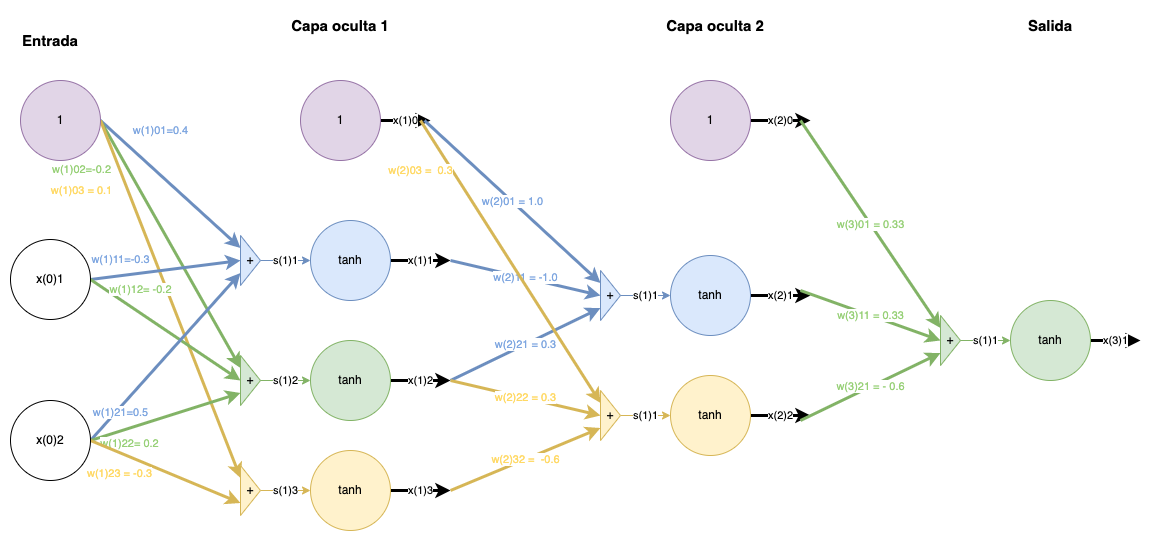
\includegraphics[width=\textwidth]{introduccion_redes_neuronales/construccion_redes_neuronales/rrnn-2-3-2-1-completa.png}
    \caption{Ejemplo de red neuronal con tres capas ocultas}
    \label{img:construccion_rrnn:rrnn-2-3-2-1}
\end{figure} 
Está compuesta por tres capas ocultas, el vector de entrada $x \in \R^2$, 
la primera capa oculta está compuesta por tres neuronas, la segunda por dos y la última, la salida por una. 
Las \textit{flechas} que conectan los nodos hacen referencia a los pesos de cada red neuronal. Por lo que para nosotros 
\begin{align}
    W^{(1)} = 
    \begin{bmatrix}
        0.4 & -0.3 & 0.5\\
        -0.2 & -0.2 & 0.2\\
        0.1 & 0 & -0.3
    \end{bmatrix} ,
    W^{(2)} = 
    \begin{bmatrix}
        1 & -1 & 0.3 & 0\\
        0.3& 0 & 0.3 & -0.6 
    \end{bmatrix} ,
    W^{(3)} = 
    \begin{bmatrix}
        0.33 & 0.33 & -0.6 \
    \end{bmatrix} 
\end{align}
Y si hacemos $x_0 = (1,0)$ y tomamos como función de activación
a la tangente hiperbólica, la ejecución del algoritmo queda reflejada en la tabla \ref{tab:construcción_rnnn:ejemplo_forward_propagation} resultando que 
$h((1,0)) = 0.439$.
\begin{table}[H]
    \begin{center}
\begin{tabular}{| c | c | c | c| }
    \hline
    Valor de $l$ &  $W^{(l)}$ & $\bigl(s^{(l)}\bigr)^T $ & $\bigl(x^{(l)}\bigr)^T$ \\ \hline
    0 & & & $(1,0)$ 
    \\ \hline
    1 & 
    $\begin{bmatrix}
        0.4 & -0.3 & 0.5\\
        -0.2 & -0.2 & 0.2\\
        0.1 & 0 & -0.3
    \end{bmatrix}$ 
    & $(0.1, -0.4, 0.1)$ & $(0.1, -0.38, 0.1)$
     \\ \hline
    2 & $\begin{bmatrix}
        1 & -1 & 0.3 & 0\\
        0.3& 0 & 0.3 & -0.6 
    \end{bmatrix}$
    & $(0.786, 0.126)$
    & $(0.656, 0.126)$
    \\ \hline
    3 & $\begin{bmatrix}
        0.33 & 0.33 & -0.6 
    \end{bmatrix}$ 
    & $(0.471)$ 
    & $(0.439)$
    \\ \hline
\end{tabular}
\caption{Ejemplo de ejecución del algoritmo de \textit{forward propagation}}
\label{tab:construcción_rnnn:ejemplo_forward_propagation}
\end{center}
\end{table}

\subsection{\textit{Backpropagation}}

Los parámetros que determinan una red neuronal son sus pesos, 
para actualizarlos utilizaremos la técnica de gradiente descendente. 
Que como ya explicamos consistía en \textit{avanzar} en dirección contraria a la del gradiente. 
\begin{equation}
    W(t+1) = w(t) - \eta \nabla E_{in}(w(t)). 
\end{equation}

Además, con el fin de reducir el coste del cálculo del gradiente, 
se utiliza el algoritmo conocido como \textit{backpropagation} que fue publicado en 
1989 en el artículo \cite{backpropagation-Hinton}. 

Sea $E_{in}(w)$ la función de error, la cual tomaremos como el error dentro de conjunto de entrenamiento, esto es,  si el conjunto 
de entrenamiento está constituido por $N$ datos de la forma $(x_n, y_n)$ con $x_n$ el vector de entrada y $y_n$ el estado o valor deseado para cualquier $n\in \{1, \ldots, N\}.$
\begin{equation}
    E_{in}(w) = \frac{1}{2} \sum^N_{n=1} e_n. 
\end{equation}
Para el cual 
\begin{equation}
    e_n = (h_w(x)- y_n)^2, 
\end{equation}
es una métrica para medir error entre, en nuestro caso  
la red neuronal $h_w$ y los valores deseados, con $w$ el vector que contiene las respectivas matrices de pesos de cada capa 
$W^{(l)} l \in \{1, \ldots, L\}.$  
%% Ejemplo 
Mostraremos un ejemplo primero antes de presentar el método general para facilitar la comprensión del algoritmo. 
% Imagen red neuronal simple
\begin{figure}[h!]
    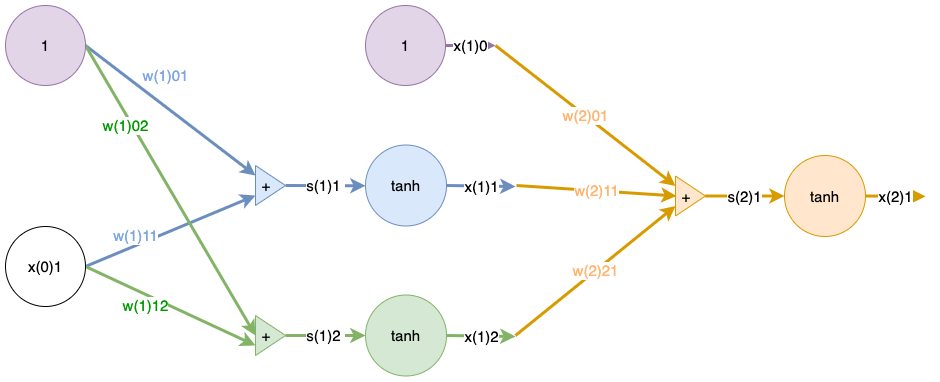
\includegraphics[width=\textwidth]{introduccion_redes_neuronales/construccion_redes_neuronales/rrnn-1-2-1.drawio.png}
    \caption{Ejemplo de red neuronal con tres capas ocultas}
    \label{img:construccion_rrnn:rrnn-1-2-1}
\end{figure} 
Queremos actualizar los pesos $w$ de la red neuronal 
$f_w : \R \longrightarrow \R$ presentada en \ref{img:construccion_rrnn:rrnn-1-2-1}.
$f_w$ está compuesta de dos capas ocultas. Supongamos que nos basaremos en un dato 
$(x, y)$ así pues podemos suponer que 
\begin{equation}
    E_{in}(w) = \frac{1}{2}e(f_w(x), y) = \frac{1}{2} (f_w(x)- y)^2.
\end{equation}
Como queremos actualizar los pesos utilizando el método de gradiente descendente necesitamos calcular el gradiente $\nabla E_{in}(w)$. 
En nuestro caso, $w=\{W^{(1)}, W^{(2)}\}$ con 
\begin{align}
    W^{(1)} = 
    \begin{bmatrix}
        w^{(1)}_{01} & w^{(1)}_{11} \\
        w^{(1)}_{02} & w^{(1)}_{12} \\
    \end{bmatrix} 
    \text{ y }
    W^{(2)} = 
    \begin{bmatrix}
        w^{(2)}_{01} & w^{(2)}_{11} & w^{(2)}_{21}\\
    \end{bmatrix}. 
\end{align}
Luego 
\begin{equation}
    \nabla E_{in}(w) = 
    \left(
        % primera capa 
        \frac{\partial e}{\partial w^{(1)}_{01}},
        \frac{\partial e}{\partial w^{(1)}_{11}},
        \frac{\partial e}{\partial w^{(1)}_{02}},
        \frac{\partial e}{\partial w^{(1)}_{12}},
        % segunda capa
        \frac{\partial e}{\partial w^{(2)}_{01}},
        \frac{\partial e}{\partial w^{(2)}_{11}},
        \frac{\partial e}{\partial w^{(2)}_{21}}
    \right).
\end{equation} 
Cada parcial se calcula, utilizando la regla de la cadena como
\begin{align}
    \frac{\partial e}{\partial w^{(1)}_{01}} 
    &=
    \frac{\partial e}{\partial s_1^{2}}
    \frac{\partial s_1^{2}}{\partial w^{(1)}_{01}} 
    \\
    &= 
    \frac{\partial }{\partial w^{(1)}_{01}}
         \tanh \left(s^{(2)}_{1}\right)
    \\
    &= 
    \left(1- \tanh^2 \left(s^{(2)}_{1}\right)\right) 
    \frac{\partial s^{(1)}_{1}}{\partial w^{(1)}_{01}}
    \\
    &= 
    \left(1- \tanh^2 \left(s^{(2)}_{1}\right)\right) 
    \frac{\partial }{\partial w^{(1)}_{01}}
    \left(w^{(2)}x^{(1)}\right)
    \\
    &= 
    \left(1- \tanh^2 \left(s^{(2)}_{1}\right)\right) 
    \frac{\partial }{\partial w^{(1)}_{01}}
    \left(
        \sum^2_{i=0}
        w^{(2)}_{i1}x^{(1)}_i
    \right)
    \\
    &= 
    \left(1- \tanh^2 \left(s^{(2)}_{1}\right)\right) 
    \left(
        \sum^2_{i=0}
        w^{(2)}_{i1}\frac{\partial x^{(1)}_i }{\partial w^{(1)}_{01}}
    \right)
    \\
    &= 
    \left(1- \tanh^2 \left(s^{(2)}_{1}\right)\right) 
    \left(
        \sum^2_{i=1}
        w^{(2)}_{i1}\frac{\partial }{\partial w^{(1)}_{01}}
        \left(
            \tanh \left(s^{(1)}_{i}\right)
        \right)
    \right)
    \\
    &= 
    \left(1- \tanh^2 \left(s^{(2)}_{1}\right)\right) 
    \left(
        \sum^2_{i=1}
        w^{(2)}_{i1}
        \left(
            \left(1- \tanh^2 \left(s^{(1)}_{i}\right)\right)
            \frac{\partial  }{\partial w^{(1)}_{01}}
            \left(
                \sum^1_{j=0}\sum^2_{k=1}
                w^{(1)}_{j k}x^{(0)}_j
            \right)
        \right)
    \right)
    \\
    &= 
    \left(1- \tanh^2 \left(s^{(2)}_{1}\right)\right) 
    \left(
        \sum^2_{i=1}
        w^{(2)}_{i1}
        \left(
            \left(1- \tanh^2 \left(s^{(1)}_{i}\right)\right)
            x^{(0)}_0
        \right)
    \right).
\end{align}
Notemos que no se han evaluado las apariciones de $s_i^{(j)}$.
Otro ejemplo sería
\begin{align}
    \frac{\partial e}{\partial w^{(2)}_{21}} 
    &=
    \frac{\partial }{\partial w^{(2)}_{21}}
         \tanh \left(s^{(2)}_{1}\right)
    \\
    &= 
    \frac{\partial }{\partial w^{(2)}_{21}}
         \tanh \left(w^{(2)}x^{(1)}\right)
    \\
    &= \left(
    1- \tanh^2 \left(s^{(2)}_{1}\right) \right)x^{(1)}_2.
\end{align}

Notemos que no se han desarrolla los términos de la forma $s^{(i)}_j$. Además si existen $Q$ pesos la complejidad del cálculo será $\mathcal{O}(Q^2)$, sin embargo, como hemos visto existen términos que se repiten en ambas ecuaciones, luego utilizando técnicas de 
programación dinámica y almacenando los valores que se repiten, 
reduciremos el coste a una complejidad de $\mathcal{O}(Q).$ Este 
algoritmo se le conoce como el de \textit{backpropagation}
basaremos su explicación en la publicada en
el artículo \cite{backpropagation-Hinton}.
%% Fin del ejemplo 
%% COMIENZA EL ARTÍCULO 

%Formalizaremos primero qué parámetros debemos estimar del gradiente.

Sea $\theta$ una función de activación derivable, 
 $L$ el número de capas ocultas, $N$ el tamaño del conjunto de entrenamiento $x^{(0)} = (1, x_1, \ldots, x_{d^{(0)}})^T$ 
siendo $x = (x_1, \ldots, x_{d^{(0)}})^T$ la entrada de la red neuronal, $x^{(L)}$ la salida de la red neuronal y 
$d^{(l)}$ la dimensión, número de nodos en la capa $l$-ésima. 
Recordemos que 
para cualquier $l \in \{1, \ldots, L\}$ con
\begin{equation}
    x^{(l)}
     = 
     \theta \left( s^{(l)}\right) 
     = 
     \theta \left( W^{(l)} x^{(l-1)}\right),
\end{equation}
y
\begin{equation}
    E(w) = \frac{1}{2} 
    \sum_{n = 1}^{N}
    \sum_{i = 1}^{d^{(L)}}
    \left({x_n}^{(L)}_i-y_{n_i} \right)^2
\end{equation}

%% Gradiente de la salida: 
Para simplificar la notación renombramos 
\begin{equation}
    E(w) = \sum^{N}_{n=1} e_n.
\end{equation}
y de ahora en adelante nos referiremos como $e$ a $e_n.$
Vamos a proceder a calcular primero los gradientes de la última capa, 
sea $w^{(L)}_{i j}$  con $j \in \{1, \ldots , d^{(L)}\}$, 
$i \in \{1, \ldots , d^{(L-1)}\}$  el peso que relaciona la salida 
$x_i ^{(L-1)}$ del  
nodo $i$ de la capa anterior con la entrada $s_j ^{(L)}$ del nodo $j$ de la última capa. 
Vamos a calcular $\frac{\partial e}{ w^{(L)}_{i j}}$ utilizando la regla de la cadena. 
\begin{equation}
    \frac{\partial{e}}{\partial w^{(L)}_{i j}}
     = 
     \frac{\partial{e}}{\partial x^{(L)}_j} 
     \frac{\partial x^{(L)}_j}{\partial s^{(L)}_j} 
     \frac{\partial s^{(L)}_j}{\partial w^{(L)}_{i j}}.
\end{equation}
Donde es fácil ver que para el tercer término
\begin{equation}\label{eq:backpropagation_s_última_capa_derivada}
    \frac{\partial s^{(L)}_{j}}{\partial w^{(L)}_{i j}}
    = 
    \frac{\partial }{\partial w^{(L)}_{i j}}
    \left(
        w^{(L)}_{\ast j } \cdot x^{(L-1)}
    \right)
    = 
    x^{(L-1)}_j
\end{equation}
Donde $w^{(L)}_{\ast j} = \left(w^{(L)}_{0 j}, w^{(L)}_{2 j}, \ldots, w^{(L)}_{d^{(L-1)} j}\right)$ representa los pesos correspondientes al nodo $j$,
 en forma de  vector fila y $x^{(L-1)} = \left(1, x ^{(L-1)}_1, \ldots, x ^{(L-1)}_{d^{(l-1)}}\right)^T$ el valor de la salida de la capa $L-1$
 en forma de vector columna.
 
 Por otro lado 
 \begin{equation}\label{eq:backpropagation_E_última_capa_derivada}
    \frac{\partial{e}}{\partial x^{(L)}_j} =
    x^{(L)}_j - y_j
 \end{equation}
 donde conocemos $x^{(L)}_j$ gracias al algoritmo de \textit{forward propagation}
 y $y_j$ la componente $j$-ésima del vector deseado en el entrenamiento.
y finalmente
\begin{equation}\label{eq:backpropagation_x_última_capa_derivada}
    \frac{\partial x^{(L)}_j}{\partial s^{(L)}_j} 
    = 
    \frac{d}{d s^{(L)}_j} 
        \theta \left( 
            s^{(L)}_j
        \right)
\end{equation}
que sabemos que se puede calcular por ser $\theta$ derivable y 
$s^{(L)}_j$ un valor conocido que ya ha sido calculado por el algoritmo de 
\textit{forward propagation.}

Por lo tanto, concluimos por 
(\refeq{eq:backpropagation_E_última_capa_derivada}),
(\refeq{eq:backpropagation_x_última_capa_derivada})
y  
(\refeq{eq:backpropagation_s_última_capa_derivada})
\begin{equation}
    \frac{\partial{e}}{\partial w^{(L)}_{i j}}
     = 
     \frac{\partial{e}}{\partial x^{(L)}_j} 
     \frac{\partial x^{(L)}_j}{\partial s^{(L)}_j} 
     \frac{\partial s^{(L)}_j}{\partial w^{(L)}_{i j}} 
    =
    \left( x^{(L)}_j - y_j \right) 
    \theta' \left( s^{(L)}_j\right)
    x^{(L)}_j.
\end{equation}
%%%% Gradiente interior 
Denotaremos por \textit{sensibilidad} a 
\begin{equation}
    \delta^{(l)} = \frac{\partial e}{ \partial s^{(l)}}.
\end{equation}

Para calcular la derivada de pesos de capas interiores 
$l \in \{1 \ldots L-1\}$
procederemos de la siguiente manera, para 
$j \in \{1, \ldots , d^{(l)}\}$ y 
$i \in \{1, \ldots , d^{(l-1)}\}$ 
\begin{equation}
    \frac{\partial{e}}{\partial w^{(l)}_{i j}}
     = 
     \frac{\partial e}{\partial s^{(l)}_j} 
     \frac{\partial s^{(l)}_j}{\partial w^{(l)}_{i j}}
    = 
    \delta^{(l)}
    \frac{\partial}{\partial w^{(l)}_{i j}}
    w^{(l) \cdot x^{(l-1)}}
    = 
    \delta^{(l)} x^{(l-1)}_i,
\end{equation}
donde  $x^{(l-1)}_i$ es conocida por el algoritmo de 
$\textit{forward propagation}$. por otra parte $\delta^{(l)}$ 
cumple que 
\begin{align}
    \delta^{(l)} 
    &= 
    \frac{\partial e}{\partial s^{(l)}}
    \\
    &= 
        \frac{\partial e}{\partial s^{(l+1)}}
        \frac{\partial s^{(l+1)}}{\partial s^{(l)}}
    \\
    &= 
    \delta^{(l+1)} 
    \otimes 
    \frac{\partial}{\partial s^{(l)}}
        \left( w^{(l)} \cdot \theta(s^{(l)})\right)
    \\
    &= 
    \delta^{(l+1)} 
    \otimes 
    w^{(l)} \cdot \theta'(s^{(l)}). 
\end{align}
\textcolor{red}{ Revisar penúltima operación.}
De esta manera a partir de las \textit{sensibilidades} de las 
capas posteriores es posible calcular las $l$-ésimas y puesto que 
la sensibilidad $\delta_{(L)}$ es conocida acabamos de determinar 
cómo calcular la derivada de todos los pesos  de manera constructiva. 
Procedemos a explicitar los cálculos. 

\subsubsection*{Algoritmo}  

El razonamiento expuesto conduce al siguiente proceso algorítmico 
para el cálculo de los gradientes. 
% pseudo código cálculo de sensibilidades 
\begin{algorithm}
    \caption{Algoritmo \textit{backpropagation} para calcular
    las sensinilidades $\delta^{(l)}$}
    \hspace*{\algorithmicindent} \textbf{Input}: un par de $(x,y)$ del conjunto de entrenamiento.  \\
    \hspace*{\algorithmicindent} \textbf{Output} 
    \begin{algorithmic}[1]
        % Forward propagation
        \STATE Se ejecuta el algoritmo de \textit{forward propagation} 
        
        con $x$ como entrada para calcular y guardar : 
        \begin{align}
            s^{(l)} \quad &\text{for } l = 1, \ldots, L;
            \\
            x^{(l)} \quad &\text{for } 0 = 1, \ldots, L;
        \end{align}
        % Inicializamos
        \STATE \COMMENT{Inicializamos sensibilidades últimas capas}
        \begin{equation}
            \delta^{(L)} \longleftarrow 2
            \left( 
                x^{(L)} - y
            \right)
            \theta' \left( s^{(L)} \right)
        \end{equation}
        \STATE 
        \COMMENT{ \textit{Backpropagation}}
        
        \For{$l = L-1$ to $1$}
        {
            \begin{equation}
                \delta^{(l)} 
                    \leftarrow
                \theta' 
                \left(
                    s^{(l)}
                \right)
                \otimes
                \left[
                    W^{(l+1)}
                    \delta^{(l+1)}
                \right]^{d^{(l)}}_1
            \end{equation}
        }
\end{algorithmic}
\end{algorithm}

%Metodología 
% !TeX root = ../../tfg.tex
% !TeX encoding = utf8
%
%*******************************************************
% Introducción artículo MFNAUA
%*******************************************************
\section{Las redes neuronales son aproximadores universales}  

Tras las definición \ref{sec:redes-neuronales-intro-una-capa} de red neuronal expuesta,
es pertinente la pregunta si tal estructura será 
capaz de aproximar con éxito una función genérica desconocida.   

Aunque las redes neuronales multicapa ya se venían aplicando con anterioridad, 
véase por ejemplo los usos expuestos durante la primera conferencia
internacional de redes neuronales de \cite{4307059} de 1987, 
no fue hasta 1989 que se descubrió formalmente su alcance.
 Tal delimitación se propuso en el artículo 
\textbf{Multilayer Feedforward Networks are Universal Approximators} \cite{HORNIK1989359}
 escrito por Kurt Hornik, Maxwell Stinchcombe y Halber White enunciando: 

\begin{teorema}\textbf{Las redes \textit{feedforward} multicapa son una clase de aproximadores universales } \label{teo:MFNAUA}
    \\
    Una red neuronal \textit{feedforward} multicapa estándar con tan solo una capa oculta y con una función de activación cualquiera es capaz de aproximar cualquier 
    función Borel medible  con dominios y codominios de dimensión finita (no necesariamente iguales) y con el nivel de precisión que se desee siempre y cuando 
    se utilicen suficientes neuronas. En este sentido las redes \textit{feedforward} multicapa son una clase de aproximadores universales.

\end{teorema}

En las secciones siguientes, con el fin de alcanzar una
 comprensión profunda de las redes neuronales,
trataremos de desgranar y profundizar en el artículo y su 
demostración. Primero precisaremos o introduciremos conceptos elementales 
sobre redes neuronales \ref{ch:articulo:sec:defincionesPrimeras}, después 
demostraremos el teorema en el caso real 
\ref{teo:TeoremaConvergenciaRealEnCompactosDefinicionesEsenciales} e iremos refinando y generalizando los resultados hasta probar
el resultado enunciado \ref{teo:MFNAUA} para una capa oculta.

 % Nota margen de denso
 \setlength{\marginparwidth}{\bigMarginSize}
 \marginpar{\maginLetterSize
     \iconoAclaraciones \textcolor{dark_green}{ 
         \textbf{Idea intuitiva conjunto denso.}
     }
     Si $S$ es denso en $T$, 
     se está está diciendo que \textbf{los elementos de $S$ son capaces de aproximar cualquier elemento de $T$
     con la precisión que se desee}. 
 }

 
El esquema general será: 

\begin{align*}
    \rrnn 
        \xRightarrow[]{\ref{teo:2_4_rrnn_densas_M}}  
    \rrnng 
        \xRightarrow[]{\ref{teorema:2_3_uniformemente_denso_compactos}}
    \pmcg
        \xRightarrow[]{\ref{teo:TeoremaConvergenciaRealEnCompactosDefinicionesEsenciales}}     
    \fC    
        \xRightarrow[]{\ref{teo:2_2_denso_función_continua}} 
    \fM.
\end{align*}

   

\begin{itemize}
    \item Las redes neuronales que nosotros hemos modelizado son densas en un espacio más general que hemos denominado \textit{Anillo de aproximación de redes neuronales}
    generado a partir de una función de activación $\psi$. 
    \item Que a su vez es denso en el \textit{Anillo de aproximación de redes neuronales}
    generado a partir de una función medible $G$. 
    \item El espacio \textit{Anillo de aproximación de redes neuronales} es denso en el de las funciones continuas.
    \item Las funciones continuas son densas en el espacio de funciones medibles. 
\end{itemize}

Si quisiéramos situar en este esquema a otras definiciones de redes neuronales las situaríamos entre  nuestro modelo y el espacio \textit{Anillo de aproximación de redes neuronales}; en  el capítulo \ref{chapter:construir-redes-neuronales} se probará tal resultado y analizarán los beneficios de basarnos en un modelo más simple. 



% !TeX root = ../../tfg.tex
% !TeX encoding = utf8
%
%*******************************************************
% Registro horas trabajo
%*******************************************************
\chapter{Registro horas de trabajo}  

Se han ido registrando las horas  de trabajo
en una hoja de cálculo \cite{TFG-hoja-calculo-horas-trabajo}
conjunto a una descripción de la tarea y los milestones relacionados. 

En total el número de horas invertidas ha sido: 

Que se distribuye de la siguiente manera en los distintos milestones: 
% --------------------------------------------------------------------
% APPENDIX: Opcional
% --------------------------------------------------------------------

\appendix % Reinicia la numeración de los capítulos y usa letras para numerarlos
\pdfbookmark[-1]{Apéndices}{appendix} % Alternativamente podemos agrupar los apéndices con un nuevo \part{Apéndices}


%% !TeX root = ../libro.tex
% !TeX encoding = utf8

\chapter{Documentación}\label{ap:documentacion}

En este apéndice se deja la documentación en estilo \emph{python} de la documentación de las distintas clases, métodos y funciones más importantes implementados en el proyecto.

\section{Selección de Modelos}

Las clases implementadas para la parte de selección de modelos que se pueden encontrar en la carpeta $PV/src$.

\subsection{Perturbated Validation}

Esta clase y sus métodos se encuentran en el archivo $PV.py$.

\paragraph{PV}

Clase PV que implementa el método para calcular y manejar la heurística PV. Guarda los datos de las series originales, las perturbaciones realizadas, los ratio de error, el nombre del dataset que se está perturbando, y valores auxiliares para imprimir gráficas del cálculo del PV.

\begin{lstlisting}
class PV:
    """
        Clase que implementa Perturbation Validation (PV).

        Attributes
        ----------
        X : np.array
            Dataset
        y : np.array
            Conjuto de etiquetas perturbadas
        ds_name : str
            Nombre del dataset
        errs : np.array
            Errores tomados
        counter : int
            Contador auxiliar
        fig : Figure
            Figura actual
        ax : Axes
            Ejes actuales
    """
\end{lstlisting}

\paragraph{Constructor}

Constructor de la clase PV que necesita los datos originales, el número de perturbaciones, el nombre del \emph{dataset}, y el inicio y fin de los ratio de error. Crea los conjuntos de etiquetas perturbadas.

\begin{lstlisting}
def __init__(self, X, y, n_pv = 5, ds_name = "", err_ini = 0.1,
                 err_fin = 0.3):
        """
            Inicializa la clase creando las etiquetas perturbadas.

            Las perturbaciones se realizan tomando un %err de cada
            clase, poniendole otra etiqueta distinta.

            Se toman "n_pv" puntos entre [err_ini, err_fin].

            Parameters
            ----------
            X : np.array
                Dataset
            y : np.array
                Etiquetas
            n_pv: int
                Número de puntos/errores
            ds_name: str
                Nombre del datases
            err_ini : float
                Error inicial
            err_fin : float
                Error final
        """
\end{lstlisting}

\paragraph{Cálculo PV}

Método para calcular el valor PV de un modelo dado.

\begin{lstlisting}
def get_pv(self, clf, clf_name = "", plot = True):
        """
            Calcula el PV score para el clasificador.

            Parameters
            ----------
            clf : Classifier
                Clasificador
            clf_name : str
                Nombre del clasificador

            Returns
            -------
            pv : float
                PV score
            accs : list(float)
                accs obtenidos
        """
\end{lstlisting}

\paragraph{Dibujar cálculo PV}

Método para representar en una gráfica los valores de la métrica $acc$ obtenidos en el cálculo de PV junto a la recta de regresión obtenida.

\begin{lstlisting}
def plot_pv(self, errs, accs, poly, pv, clf_name = ""):
        """
            Dibuja los puntos y la recta de regresión en la figura actual.

            Parameters
            ----------
            errs : np.array
                Errores
            accs : np.array
                acc obtenidos
            poly : np.array
                Recta de regresión
            pv : float
                Valor PV
            clf_name : str
                Nombre del clasificador
        """
\end{lstlisting}

\paragraph{Guardar gráfica}

Método para guardar en una imagen .png el gráfico del método $plot\_pv$.

\begin{lstlisting}
def save_graph(self, name_fig):
        """
            Guarda el gráfico de los resultados en un .png

            Parameters
            ----------
            name_fig : str
                Nombre (ruta) de la imagen a guardar.
        """
\end{lstlisting}

\subsection{Clasificador LSTM}

Esta clase y sus métodos se encuentran en el archivo $LSTM.py$.

\paragraph{LSTM}

La clase LSTM que implementa el clasificador LSTM. Guarda el modelo LSTM, el número de clases, la longitud de las series, opciones de entrenamiento y para gráficas de entrenamiento.

\begin{lstlisting}
class LSTM(BaseEstimator):
    """
        Implementación de una red neuronal con capas LSTM.

        Attributes
        ----------
        counter : int, static
            Valor auxiliar para ruta de imagen
        model : Sequential
            Modelo red neuronal
        history : list
            Historial del entrenamiento
        n_clases : int
            Número de clases de las etiquetas
        input_shape : tuple
            Forma de los datos
        epochs: int
            Número de épocas para entrenamiento
        verbose : int
            Información sobre el entrenamiento
        save_hist : boolean
            Si guardar las gráficas de los entrenamientos
    """
\end{lstlisting}

\paragraph{Constructor}

Constructor de la clase LSTM que guarda opciones de entrenamiento.

\begin{lstlisting}
def __init__(self, epochs, n_neurs = 80, verbose = 0, save_hist = False,
             n_clases = -1):
        """
            Inicializamos la red LSTM.

            Attributes
            ----------
            epochs : int
                Número de épocas para entrenamiento
            n_neurs : int
                Número de neuronas LSTM
            verbose : int
                Información sobre el entrenamiento
            save_hist : boolean
                Si guardar las gráficas de los entrenamientos
            n_clases : int
                Número de clases a predecir
        """
\end{lstlisting}

\paragraph{Creación del modelo}

Método para crear el modelo LSTM.

\begin{lstlisting}
def create_model(self):
        """
            Crea el modelo LSTM.
        """
\end{lstlisting}

\paragraph{Compilar el modelo}

Compila el modelo con el optimizador ADAM y la función de pérdida entropía cruzada categórica.

\begin{lstlisting}
def compile_model(self):
        """
            Compila el modelo con optimizador ADAM y función de pérdida
            categorical_crossentropy.
        """
\end{lstlisting}

\paragraph{Entrenamiento}

Método para entrenar el modelo con el conjunto de datos, con las épocas guardadas, validación al 10\% y con parada temprana.

\begin{lstlisting}
def fit(self, X, y):
        """
            Entrenamos el modelo.

            Parameters
            ----------
            X : numpy.array
                Datos de entrenamiento
            y : numpy.array
                Etiquetas de entrenamiento
        """
\end{lstlisting}

\paragraph{Cálculo métrica}

Método para calcular la métrica $acc$ en el conjunto de datos pasado.

\begin{lstlisting}
def score(self, X, y):
        """
            Calcula el acc con los datos que se le pasan.

            Parameters
            ----------
            X : numpy.array
                Datos test
            y : numpy.array
                Etiquetas test

            Returns
            ----------
            acc : float
                accuracy obtenida
        """
\end{lstlisting}

\paragraph{Guardar gráfica de entrenamiento}

Método para guardar el historial de entrenamiento en una imagen.

\begin{lstlisting}
def save_history(self):
        """
            Guarda el historial en una imagen.
        """
\end{lstlisting}

\subsection{Clasificadores}

Los clasificadores adicionales que usamos para comparar modelos, comparten dos métodos generales: entrenamiento y cálculo de la métrica.

\paragraph{Entrenamiento}

Método que se encarga de entrenar el modelo usando una muestra de datos.

\begin{lstlisting}
def fit(self, X, y):
    """
        Entrena el modelo.

        Parameters
        ----------
        X : numpy.array
            Datos de entrenamiento
        y : numpy.array
            Etiquetas de entrenamiento
    """
\end{lstlisting}

\subparagraph{Cálculo de métrica}

Método que se encarga de calcular la métrica ($accuracy$) de un modelo en un conjunto de datos.

\begin{lstlisting}
def score(self, X, y):
    """
        Calcula el acc con los datos que se le pasan.

        Parameters
        ----------
        X : numpy.array
            Datos test
        y : numpy.array
            Etiquetas test

        Returns
        ----------
        acc : float
            accuracy obtenida
    """
\end{lstlisting}

\subsubsection{C4.5}

Esta clase y sus métodos se encuentran en el archivo $RClassifiers.py$.

\paragraph{C45}

La clase C45 que usa el árbol de decisión C4.5 que guarda el modelo.

\begin{lstlisting}
class C45(BaseEstimator):
    """
        Implementa el árbol de decisión C4.5.

        Attributes
        ----------
        model : clasificador en R
            El clasificador (clase en R)
    """
\end{lstlisting}

\subsubsection{C5.0}

Esta clase y sus métodos se encuentran en el archivo $RClassifiers.py$.

\paragraph{C50}

La clase C50 que usa el árbol de decisión C5.0 que guarda el modelo, y también el valor del \emph{boosting}.

\begin{lstlisting}
class C50(BaseEstimator):
    """
        Implementa el árbol de decisión C5.0 (con boosting o no).

        Attributes
        ----------
        model : clasificador en R
            El clasificador (clase en R)
        boosting : int
            El valor del boosting
    """
\end{lstlisting}

\paragraph{Constructor}

Constructor de la clase C50 que se le pasa el número de \emph{boosting} que se necesite.

\begin{lstlisting}
def __init__(self, boosting = 10):
        """
            Inicializa el clasificador.

            Parameters
            ----------
            boosting : int
                El valor del boosting
        """
\end{lstlisting}

\subsubsection{Recursive Partioning Tree}

Esta clase y sus métodos se encuentran en el archivo $RClassifiers.py$.

\paragraph{RPart}

Clase que usa el árbol RPart.

\begin{lstlisting}
class RPart(BaseEstimator):
    """
        Implementa el árbol de decisión RPart (Recursive Partioning Tree).

        Attributes
        ----------
        model : clasificador en R
            El clasificador (clase en R)
    """
\end{lstlisting}

\subsubsection{Condicional Tree}

Esta clase y sus métodos se encuentran en el archivo $RClassifiers.py$.

\paragraph{CTree}

La clase CTree implementa el uso del árbol de decisión Condicional Tree.

\begin{lstlisting}
class CTree(BaseEstimator):
    """
        Implementa el árbol de decisión CTree (Conditional Inference Tree).

        Attributes
        ----------
        model : clasificador en R
            El clasificador (clase en R)
    """
\end{lstlisting}


\subsubsection{$k$-NN}

Esta clase y sus métodos se encuentran en el archivo $KNN.py$.


\paragraph{Clase KNN}

Clase que implementa el clasificador $k$-NN que se le puede pasar el $k$ fijo o que lo calcule automáticamente tomado como la raíz cuadrada del número de datos.

\begin{lstlisting}
class KNN(BaseEstimator):
    """
        Implementa el clasificador KNN (K-Nearest neighbors).

        Parameters
        ----------
        k : int
            Número de vecinos
        model : KNeighborsClassifier
            Modelo k-NN
        metric : str, metric
            Métrica que usar con KNN
        n_jobs : int
            Número de procesadores usados
    """
\end{lstlisting}

\paragraph{Constructor}

Constructor de la clase KNN que necesita el número de vecinos, la métrica y el número de procesadores.

\begin{lstlisting}
def __init__(self, k = None, metric = "euclidean", n_jobs = 1):
        """
            Inicializa el clasificador.

            Parameters
            ----------
            k : int
                Número de vecinos
            metric : str, metric
                Métrica que usar con KNN
            n_jobs : int
                Número de procesadores
        """
\end{lstlisting}

\subsubsection{$k$-NN + DTW}

Esta clase y sus métodos se encuentran en el archivo $RClassifiers.py$.

\paragraph{DTW}

Clase que implementa el clasificador $k$-NN con métrica DTW, que guarda los datos de entrenamiento, el número de vecinos y el tamaño de la ventana para aplicar DTW.

\begin{lstlisting}
class DTW(BaseEstimator):
    """
        Clase que implementa K-Nearest Neighbors con la distancia DTW
        usando la implementación del paquete "IncDTW".

        Attributes
        ----------
        data : R.DataFrame
            Datos transformados en un objeto dataframe de R
        k : int
            Número de vecinos
        window_shift : int
            Tamaño de la ventana para aplicar DTW
    """
\end{lstlisting}

\paragraph{Constructor}

Constructor de la clase DTW que necesita el número de vecinos y el tamaño de la ventana para el cálculo de la métrica DTW.

\begin{lstlisting}
def __init__(self, k = 1, window_shift = 5):
    """
        Constructor de la clase, debe hacerse solo una vez por dataset.

        Parameters
        ----------
        k : int
            Números de vecinos
        window_shift : int
            Tamaño de la ventana para aplicar DTW
    """
\end{lstlisting}

\section{Detección de anomalías}

Funciones y clases relativas a la parte de detección de anomalías que se encuentran en la carpeta $AD/src$.

\subsection{Alteración de series}

Funciones para la creación de anomalías en base a las series normales implementadas en el archivo $alteraciones.py$.

\paragraph{Tramo aleatorio}

Función para escoger un tramo aleatorio de la serie en función a la longitud indicada (máxima, mínima, fija).

\begin{lstlisting}
def random_slice(x, max_length = None, min_length = None,
                   length = None, pos = None, border = 0):
    """
        Se encarga de elegir un tramo aleatorio de una serie que queda
        determinado por una posición y longitud, de manera que el tramo
        elegido es [posición, posición + longitud).

        Se puede determinar una longitud máxima o mínima, o incluso
        especificar una longitud o posición fijada. También se puede
        indicar si excluir los extremos (añadir borde).

        Parameters
        ----------
        x : np.numpy
            Serie temporal que alterar
        max_length : int, None
            Longitud máxima de la perturbación
        min_length : int, None
            Longitud mínima de la perturbación
        length : int, None
            Longitud fija de la perturbación
        pos : int, None
            Posición fija de la perturbación
        border : int
            Borde para excluir la perturbación

        Returns
        -------
        pos : int
            Posición de la perturbación
        length : int
            Longitud de la perturbación
    """
\end{lstlisting}

\paragraph{Ruido gaussiano}

Método para alterar un tramo aleatorio de la serie añadiendo ruido gaussiano mediante un parámetro $\sigma$ que controla la intensidad de esta perturbación, y la longitud máxima y mínima de esta.

\begin{lstlisting}
def gaussian_noise(x, max_length, min_length = 3, std = 3, neg = False,
                   border = 0, neg_random = True):
    """
        Crea una perturbación de ruido gaussiano añadiendo en un
        tramo aleatorio un muestreo de la función de densidad normal.
        Se puede controlar la intensidad.

        Además se puede activar aleatoriamente (50%) o de manera fija que la
        alteración gaussiana sea negativa.

        Parameters
        ----------
        x : np.numpy
            La serie para alterar
        max_length : int
            Longitud máxima de la alteración
        min_length : int
            Longitud minima de la alteración
        std : float
            Controla la intensidad de la alteración
        neg : boolean
            Si invertir la señal gaussiana
        border : int
            El borde para excluir la perturbación
        neg_random : boolean
            Si se invierte aleatoriamente las señales

        Returns
        -------
        x : np.numpy
            Una copia de la señal perturbada
    """
\end{lstlisting}

\paragraph{Pulso sinusoidal-gaussiano}

Método para alterar un tramo aleatorio de la serie añadiendo un pulso sinusoidal-gaussiano mediante su frecuencia $fc$, un parámetro $\sigma$ que controla la intensidad de la perturbación y la longitud máxima y mínima de esta.

\begin{lstlisting}
def gaussian_sine_pulse(x, max_length, min_length = 3, fc = 1.5, std = 3,
                        border = 0):
    """
        Crea una perturbación con un pulso sinusoidal-gaussiano añadido en un
        tramo aleatorio. Se puede controlar la intensidad y la frecuencia
        del pulso.

        Parameters
        ----------
        x : np.numpy
            La serie para alterar
        max_length : int
            Longitud máxima de la alteración
        min_length : int
            Longitud minima de la alteración
        fc : float
            Frecuencia de la señal del pulso
        std : float
            Controla la intensidad de la alteración
        border : int
            El borde para excluir la perturbación

        Returns
        -------
        x : np.numpy
            Una copia de la señal perturbada
    """
\end{lstlisting}

\paragraph{Estacionalidad}

Método para alterar un tramo aleatorio de la serie modificando la estacionalidad de la descomposición STL (dada con un periodo) por un parámetro $\sigma$ que controla la intensidad y la longitud máxima y mínima de esta.

\begin{lstlisting}
def modify_season(x, period, max_length, min_length = 3, std = 1, border = 0):
    """
        Crea una perturbación multiplicando por un real la estacionalidad
        de un tramo aleatorio de la serie. Se necesita el periodo para
        realizar la descomposición STL.

        Parameters
        ----------
        x : np.numpy
            La serie para alterar
        period : int
            Periodo de repetición de la serie para descomposición STL
        max_length : int
            Longitud máxima de la alteración
        min_length : int
            Longitud minima de la alteración
        std : float
            Controla la intensidad de la alteración
        border : int
            El borde para excluir la perturbación
    """
\end{lstlisting}

\paragraph{Tendencia}

Método para alterar un tramo aleatorio de la serie modificando la tendencia de la descomposición STL (dada con un periodo) por un parámetro $\sigma$ que controla la intensidad y la longitud máxima y mínima de esta.

\begin{lstlisting}
def modify_trend(x, period, max_length, min_length = 3, std = 1, border = 0):
    """
        Crea una perturbación multiplicando por un real la tendencia
        de un tramo aleatorio de la serie. Se necesita el periodo para
        realizar la descomposición STL.

        Parameters
        ----------
        x : np.numpy
            La serie para alterar
        period : int
            Periodo de repetición de la serie para descomposición STL
        max_length : int
            Longitud máxima de la alteración
        min_length : int
            Longitud minima de la alteración
        std : float
            Controla la intensidad de la alteración
        border : int
            El borde para excluir la perturbación
    """
\end{lstlisting}

\subsection{Detector}

Clase y sus métodos implementados para crear el detector de anomalías, implementado en $detector.py$

\paragraph{Clase LSTM\_AD}

Clase que implementa el detector de anomalías basado en autoencoder LSTM. Mantiene el modelo LSTM, la probabilidad estimada y otros parámetros de entrenamiento.

\begin{lstlisting}
class LSTM_AD:
    """
        Clase que implementa un detector de anomalías usando
        un modelo autoencoder con capas LSTM.

        Attributes
        ----------
        model : keras.Sequential
            Autoencoder LSTM
        n_neur : int
            Número de neuronas base para las capas
        alpha : float
            Parámetro de regularización L2
        lr : float
            Learning rate
        epochs : int
            Número de épocas de entrenamiento
        mode : int
            Si incluir espacio de codificación (1) o no (2)
        hist : keras.Historial
            Historial de entrenamiento
        kernel : scipy.gaussian_kde
            Distribución de errores estimada
    """
\end{lstlisting}

\paragraph{Constructor}

Constructor de la clase LSTM\_AD que guarda los parámetros relativos al entrenamiento y al modo de arquitectura.

\begin{lstlisting}
def __init__(self, n_neur = 32, alpha = 0, lr = 0.001, epochs = 300,
             mode = 2):
    """
        Constructor de la clase

        Parameters
        ----------
        n_neur : int
            Número de neuronas base para las capas
        alpha : float
            Parámetro de regularización L2
        lr : float
            Learning rate
        epochs : int
            Número de épocas de entrenamiento
        mode : int
            Si incluir espacio de codificación (1) o no (2)
    """
\end{lstlisting}

\paragraph{Creación del modelo}

Función para crear la arquitectura del modelo autoencoder LSTM.

\begin{lstlisting}
def create_model(self, X):
    """
        Crea la arquitectura del autoencoder LSTM con los atributos
        de la clase.

        Parameters
        ----------
        X : np.numpy
            Series temporales
    """
\end{lstlisting}

\paragraph{Compilación}

Función para compilar el modelo autoencoder LSTM.

\begin{lstlisting}
def compile_model(self):
    """
        Compila el modelo con ADAM añadiendo un clip de 1, learning
        rate especificado y minimizando el error cuadrático medio.
    """
\end{lstlisting}

\paragraph{Entrenamiento}

Función para entrenar el modelo autoencoder LSTM.

\begin{lstlisting}
def load_model(self, path):
    """
        Carga el modelo de unos pesos guardados en un archivo

        Parameters
        ----------
        path : str
            Ruta donde está el archivo de los pesos
    """
\end{lstlisting}

\paragraph{Reconstrucción}

Función para obtener las reconstrucciones de un conjunto de series temporales.

\begin{lstlisting}
"""
    Obtiene las reconstrucciones del autoencoder para las series.

    Parameters
    ----------
    X : numpy.array
        Datasets de series temporales

    Returns
    -------
    reconstrucciones : numpy.array
        Reconstrucciones de las series temporales
"""
\end{lstlisting}

\paragraph{Estimar distribución}

Función para estimar la distribución de los errores de reconstrucción.

\begin{lstlisting}
def fit_kernel(self, X):
    """
        Ajustamos la distribución de los errores de reconstrucción
        con los datos de entrenamiento.

        Parameters
        ----------
        X : numpy.array
            Dataset de series temporales
    """
\end{lstlisting}

\paragraph{Calcular probabilidades}

Función para obtener las probabilidades de ser serie anómala para un conjunto de series temporales.

\begin{lstlisting}
def predict_prob(self, X):
    """
        Devolvemos las probabilidades de ser serie anómala para
        cada serie del dataset

        Parameters
        ----------
        X : numpy.array
            Dataset de series temporales

        Returns
        -------
        probs : numpy.array
            Probabilidades de anomalía para cada serie
    """
\end{lstlisting}

\subsection{Cálculo Curva Precision-Recall}

Las funciones para calcular la métrica $AUC$-$PR$ (curva precisión-recall) que se encuentran en el archivo $calc\_pr.py$.

\paragraph{Contar anomalías}

Se cuentan el número de anomalías detectadas en función de las probabilidades de las series de ser anómalas y de un umbral de probabilidad al partir del cual se considera que es anómala.

\begin{lstlisting}
def count_anomalies(probs, threshold):
    """
        Cuenta cuantas anomalías hay en función a la probabilidad de serlo
        y un umbral de probabilidad.

        Parameters
        ----------
        probs : np.numpy
            Array con probabilidades de cada serie de ser anómala
        threshold : float
            Umbral de probabilidad a partir del cual se considera anómala

        Returns
        -------
        n_anomalies : int
            Número de anomalías detectadas
    """
\end{lstlisting}

\paragraph{Calcular sensibilidad}

Se calcula la sensibilidad del modelo en base a las probabilidades de las series anómalas y un umbral.

\begin{lstlisting}
def calc_recall(probs_anomalies, threshold):
    """
        Calcula la sensibilidad (recall) de un modelo en base a las
        probabilidades de las series anómalas.

        Parameters
        ----------
        probs_anomalies : np.numpy
            Array con probabilidades de anomalías de las series anómalas
        threshold : float
            Umbral de probabilidad

        Returns
        -------
        recall : float
            Sensibilidad del modelo
    """
\end{lstlisting}

\paragraph{Calcular precisión}

Se calcula la precisión del modelo en base a las probabilidades de las series anómalas y normales junto a un umbral.

\begin{lstlisting}
def calc_precision(probs_normal, probs_anomalies, threshold):
    """
        Calcula la precisión de un modelo en base a las probabilidades
        de las series anómalas y normales.

        Parameters
        ----------
        probs_normal : np.numpy
            Array con probabilidades anomalías de las series normales
        probs_anomalies : np.numpy
            Array con probabilidades anomalías de las series anómalas
        threshold : float
            Umbral de probabilidad

        Returns
        -------
        precision : float
            Precisión del modelo
    """
\end{lstlisting}

\paragraph{Curva Precision-Recall}

Se calcula la métrica $PR$ tomando el área debajo de la curva Precision-Recall integrando en el cuadrado $[0, 1]^2$. Además se imprime una figura mostrando la curva que se forma.

\begin{lstlisting}
def recall_precision_curve(X_normal, X_anomalies, model, clf_name = "clf",
                           title = "recall-precision curve", axis = None,
                           plot = True):
    """
        Calcula la métrica PR y además muestra la curva Precision-Recall
        del modelo.

        Parameters
        ----------
        X_normal : np.numpy
            Series normales
        X_anomalies : np.numpy
            Series anómalas
        model : detector
            Detector de anomalías
        clf_name : str
            Nombre del detector
        title : str
            Título de la gráfica
        axis : matplotlib.axis
            Objeto para imprimir las gráficas
        plot : boolean
            Si imprimir cosas opcionales de la gráfica

        Returns
        -------
        pr_score : float
            Valor de la métrica PR
    """
\end{lstlisting}


\endinput
%------------------------------------------------------------------------------------
% FIN DEL APÉNDICE.
%------------------------------------------------------------------------------------


% Añadir tantos apéndices como sea necesario

% --------------------------------------------------------------------
% GLOSARIO: Opcional
% --------------------------------------------------------------------

%\include{glosario}


% -------------------------------------------------------------------
% BACKMATTER
% -------------------------------------------------------------------

\backmatter % Desactiva la numeración de los capítulos
\pdfbookmark[-1]{Referencias}{BM-Referencias}

% BIBLIOGRAFÍA
%-------------------------------------------------------------------

\setbibpreamble{Las referencias se listan por orden alfabético. Aquellas referencias con más de un autor están ordenadas de acuerdo con el primer autor.\par\bigskip}
\bibliographystyle{alphaurl}
\begin{small} % Normalmente la bibliografía se imprime en un tamaño de letra más pequeño.
\bibliography{library.bib}
\end{small}


% ÍNDICE TERMINOLÓGICO  (Opcional)
%-------------------------------------------------------------------

\cleardoublepage
\begin{footnotesize} % Normalmente el índice se imprime en un tamaño de letra más pequeño.
\printindex
\end{footnotesize}
% !TeX root = ../libro.tex
% !TeX encoding = utf8

%*******************************************************
% Agradecimientos
%*******************************************************

\chapter*{Agradecimientos}

Agradezco a 
\endinput

\end{document}
